\documentclass[a4paper,openany]{book}
\usepackage{MyStyle}
\usepackage{CodeStyle}

\hypersetup{
  pdftitle={DDLC Mod开发指南},
  pdfkeywords={DDLC, Mod},
  pdfcreator={PartyParrot},
}

\makeindex

\begin{document}

% \pagenumbering{Alph}
\pagenumbering{Alph}
\begin{titlepage}{

\newcommand{\version}{0.1.0}

\begin{figure}
    
\includegraphics[scale=.1]{Pictures/封面/logo}
\end{figure}

\vspace*{\stretch{1}}


\noindent\begin{minipage}{\textwidth}
\raggedright
{\fontsize{60pt}{1.2} \bfseries DDLC Mod}
\newline
\newline
{\fontsize{50pt}{1.2} \bfseries 开发指南}
\noindent\rule[-1ex]{\textwidth}{5pt}\\[2.5ex]
\Large {DDLC MOD Development Guide\newline} \hfill

{\bfseries \fontsize{15pt}{1.2}{(Ver. \version)}}
\newline
{\bfseries \fontsize{15pt}{1.2}{PartyParrot 著}}
\end{minipage}

\vspace{\stretch{2}}

\newpage
\begin{quote}\footnotesize\large
DDLC Mod Development Guide {\copyright} 2023 - {\the\year} by PartyParrot is licensed under CC BY-NC-SA 4.0.

PartyParrot 所著的DDLC Mod开发指南 {\copyright} 2023 - {\the\year}基于CC BY-NC-SA 4.0分发。
\end{quote}
}
\end{titlepage}

% \title{\Huge \sffamily \bfseries{DDLC Mod 开发指南}}
% \author{\huge \sffamily PartyParrot}
% \date{\sffamily \today}
% \maketitle

\frontmatter
\chapter{前言}

Ren'Py是一种视觉小说语言。{\itshape 《心跳!心跳!文学部!》(Doki Doki Literature Club!},下文简称DDLC)正是基于Ren'Py编写的。因此,要编写DDLC的 Mod 就必须学习 Ren'Py。本书旨在通过简单明了的例子教会读者DDLC Mod的开发。另外,由于Ren'Py与Python是密不可分的,本书在介绍 Ren'Py 7的同时也会介绍部分Python知识。
本书中部分内容对于部分读者可能会有一定的编程门槛,请善用百度。

\subsubsection*{实例代码}
本书包含大量的示例代码,由于 Ren'Py 的特殊性,大部分代码需要放在相应环境中才能运行。本书代码只适用于 Ren'Py 7/8,大部分代码理论上可以在 Ren'Py 6 上运行,但由于其过时性,本书将不再针对 Ren'Py 6 进行介绍与适配。

\subsubsection*{本书示例代码及注释样式}
为区别普通文本,本书对于实例代码做出以下规定:
\begin{itemize}
    \item 代码英文使用 Hack 字体,中文使用思源等宽字体,字号为 14 点。背景为 (235, 235, 235)。如:
    \begin{lstlisting}[numbers=none]
# 这是一行注释
    \end{lstlisting}

    \item 需要您输入的内容将以粗体出现。如:
    \begin{lstlisting}
$ renpy.input()
%\UserInput{22}%
    \end{lstlisting}

    \item 表示代码输出结果的将以斜体出现。如:
    \begin{lstlisting}
>>> 1 + 2
%\Output{3}%
    \end{lstlisting}

    \item 语法中的占位符将用尖括号括起来。您应使用实际的参数、变量等替换占位符。如:
    \begin{lstlisting}[numbers=none]
define <变量名称> = <值:整型、浮点型等>
    \end{lstlisting}
    您应将其替换类似的例子:
    \begin{lstlisting}[numbers=none]
define a = 2
    \end{lstlisting}

    \item 当代码中不含有>>>或...则表示您应该使用文件运行代码,而非Python交互模式。

    \item 本书中只能在Python代码块中运行的语法,将会含有\PyOnly 标签。如下例:


    for循环 \PyOnly


    同时,本书分为5种注释类型:
    \item 普通注释背景使用25\%色调青色,边框使用75\%青色,如:
    \begin{Comment}
这是一行注释。
    \end{Comment}
    \item 扩展知识背景使用25\%色调绿色,边框使用RGB颜色(105, 190, 78)如:
    \begin{ExtraKnowledge}
    这是一行扩展知识。
    \end{ExtraKnowledge}
    \item 警告背景使用25\%色调黄色,边框使用RGB颜色(150, 150, 0)如:
    \begin{Warning}
    这是一行警告。
    \end{Warning}
    \item 必须注意的内容背景使用25\%色调红色,边框使用75\%红色,如:
    \begin{Attention}
    您必须注意此内容。
    \end{Attention}
\end{itemize}

\subsubsection*{获取最新版指南}
\url{https://wwyc.lanzouq.com/b02fb2saj}

密码 :ddlc

\url{https://github.com/DanilJeston/DDLC-Chinese-Modding-Guide}

\subsubsection*{联系方式}
我们的联系邮箱是: \url{team_ninety@outlook.com}。
\newline\newline\par
如果您对本书有任何疑问或建议,请发邮件给我们。若您有兴趣参与本书的编写、完善,可以邮件给我们。同时,若您发现有人未经 CC BY-NC-SA 4.0 方式分发本书,请发邮件给我们。若本书存在部分代码出现错误、无法运行等,请发送邮件给我们。

最后,祝您学习愉快!
\tableofcontents

\mainmatter
\part{基础篇}
\chapter{预备知识}
Ren'Py是一种视觉小说语言,名字是恋愛(れんあい,即恋爱)与Python两词混合而成。Python是Ren'Py使用的编程语言。而 \textit{《心跳!心跳!文学部!》(Doki Doki Literature Club!},下文简称DDLC)正是基于Ren'Py编写的。想要编写DDLC Mod,我们就必须先学习Ren'Py相关知识。

本章将为您介绍Ren'Py的来源及如何安装Ren'Py与代码编辑器。

\section{关于Ren'Py}
\subsection{Ren'Py概述}
Ren'Py几乎支持视觉小说所应该具有的功能,如:分支故事、存储与加载游戏、回退到之前故事的存储点、多样性的场景转换等。其首次发布于2004年8月24日。Ren'Py拥有类似电影剧本的语法,并且能够允许用户编写Python代码来增加新的功能。除此之外,游戏引擎内附的出版工具能提供基本的脚本加密与压缩游戏素材。

Ren'Py建构于Python软件库Pygame之上,而它又基于了SDL。Ren'Py官方支持Windows、Linux以及较新版Mac OS X,并可通过Arch Linux、Ubuntu、Debian或Gentoo的软件包管理系统安装。它可以在Windows、macOS、Linux、Android、OpenBSD、iOS和wasm的HTML5下建置。

利用Ren'Py结合剧本及Python,我们可以制作出各种各样的游戏。Ren'Py也有一些电子角色扮演游戏框架的示例,但相对来说,制作RPG游戏会比较困难。

\section{下载Ren'Py}
\label{1.2}
目前主流的Ren'Py分为3个版本:Ren'Py 6、Ren'Py 7、Ren'Py 8。其中Ren'Py 6与Ren'Py 7兼容Python 2且Ren'Py 7已经支持大部分Python 3特性,而Ren'Py 8完全兼容Python 3。需要注意的是,Ren'Py 6已停止支持。

Ren'Py几乎可在所有主流系统上运行。由于Ren'Py 8目前稳定性存疑,故本书主要使用Ren'Py 7进行教学。

\begin{Comment}
Ren'Py 7.4.4及以后的版本均不支持Windows XP及更早的系统。
\end{Comment}

\subsection{下载Ren'Py SDK 7}\label{sec:2.2.1}
\begin{figure}[htbp]
    \centering
    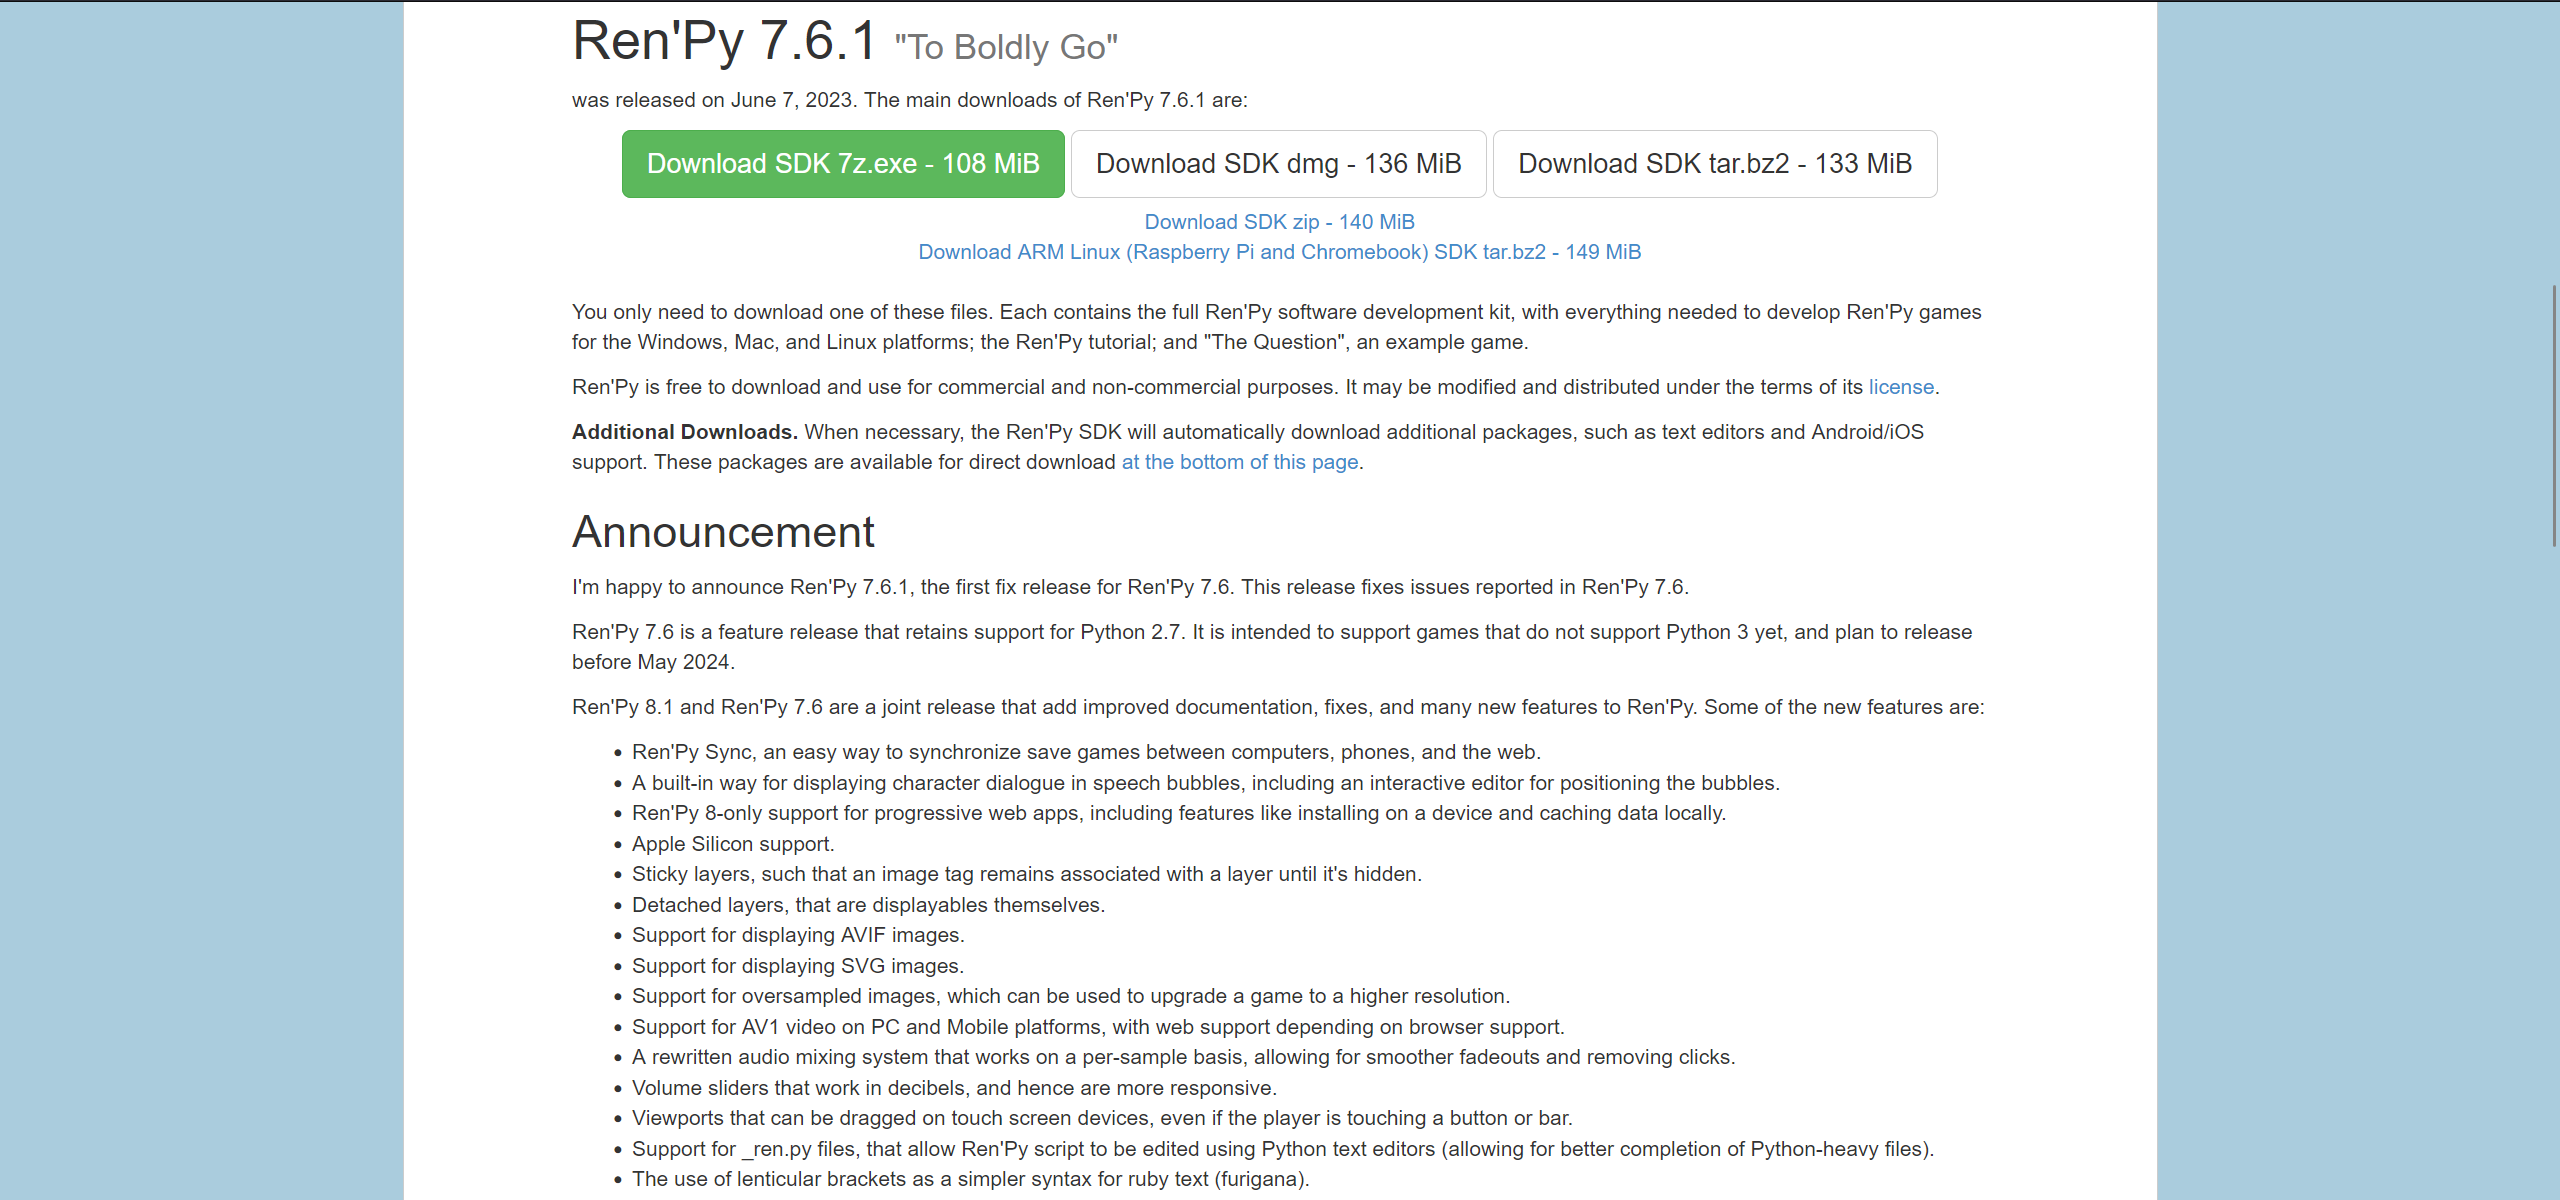
\includegraphics[scale=.3]{Pictures/1/1.2/1.2.1}
    \caption{Ren'Py官网}
    \label{fig:2.2.1}
\end{figure}

\begin{Comment}
本章编写时DDLC Mod中文模板支持的最新版Ren'Py SDK 7为7.6.1。
\end{Comment}
使用任意浏览器进入 \url{https://www.renpy.org/release/7.6.1} 网页(如图\ref{fig:2.2.1}),您将在本页面看到三个按钮,分别是:Download SDK 7z.exe、Download SDK dmg与 Download SDK tar.bz2。Windows用户请下载第一个,macOS用户请下载第二个,Linux用户请下载第三个。

\begin{Comment}
    若无法打开文件,请点击第二行小字Download SDK zip下载ZIP文件
\end{Comment}

\begin{figure}[htbp]
    \begin{minipage}{200pt}
        \centering
        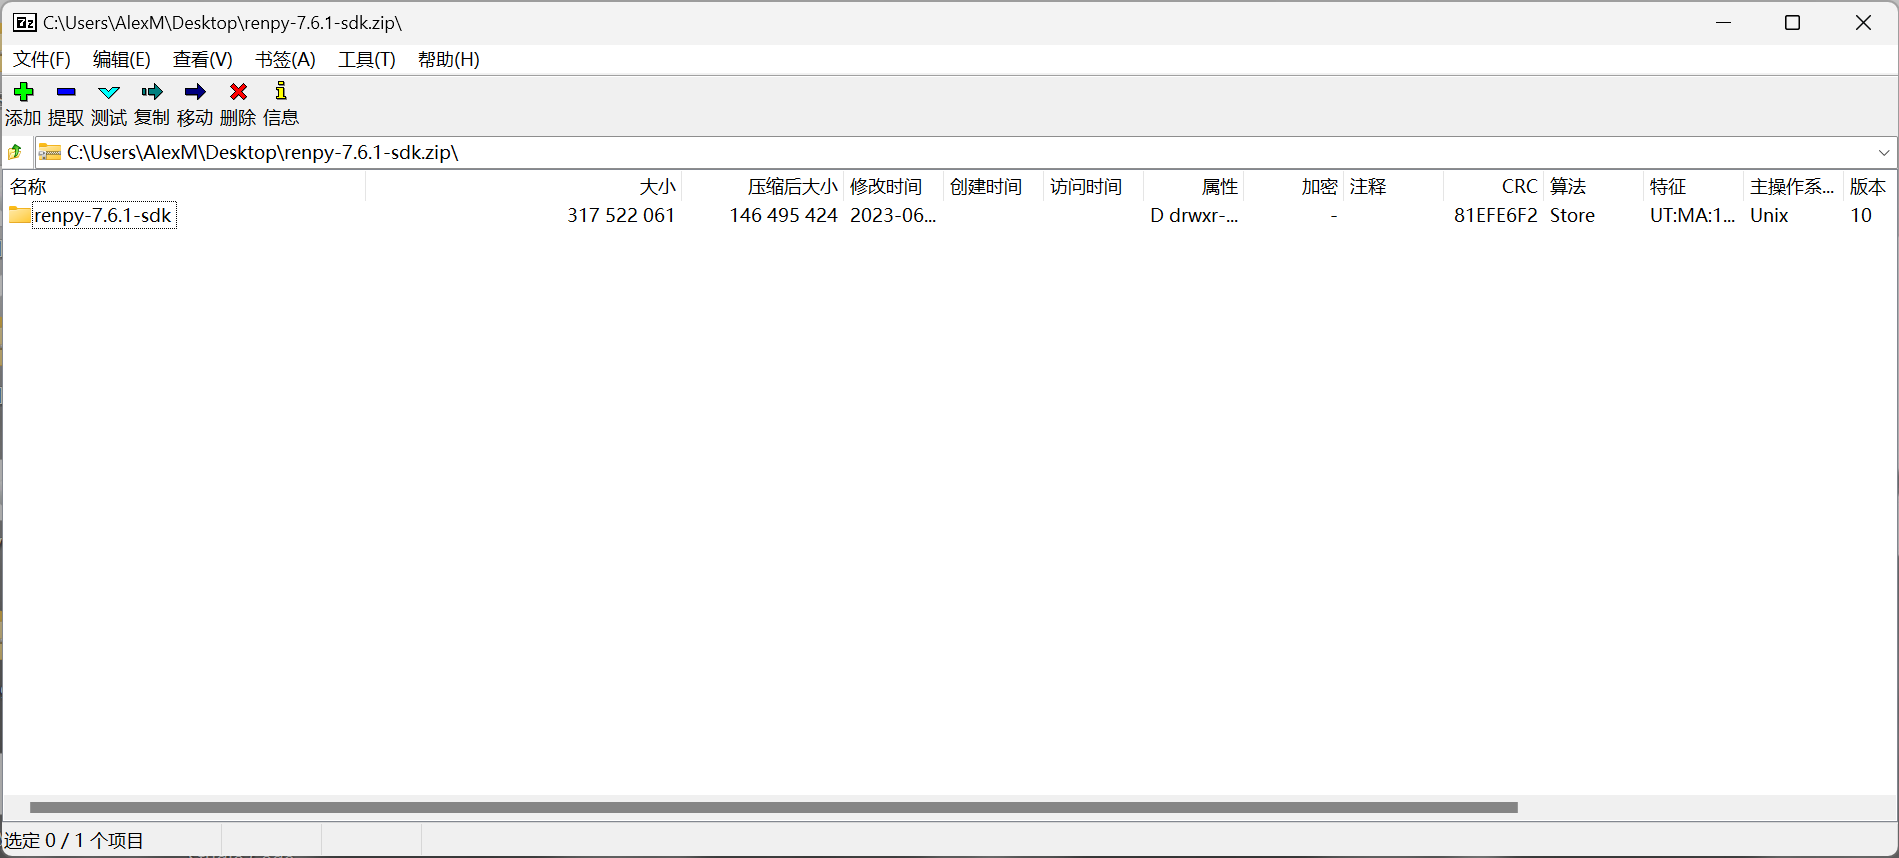
\includegraphics[scale=.2]{Pictures/1/1.2/1.2.2.png}
        \caption{ZIP文件}
        \label{fig:2.2.2}
    \end{minipage}
    \begin{minipage}{180pt}
        \centering
        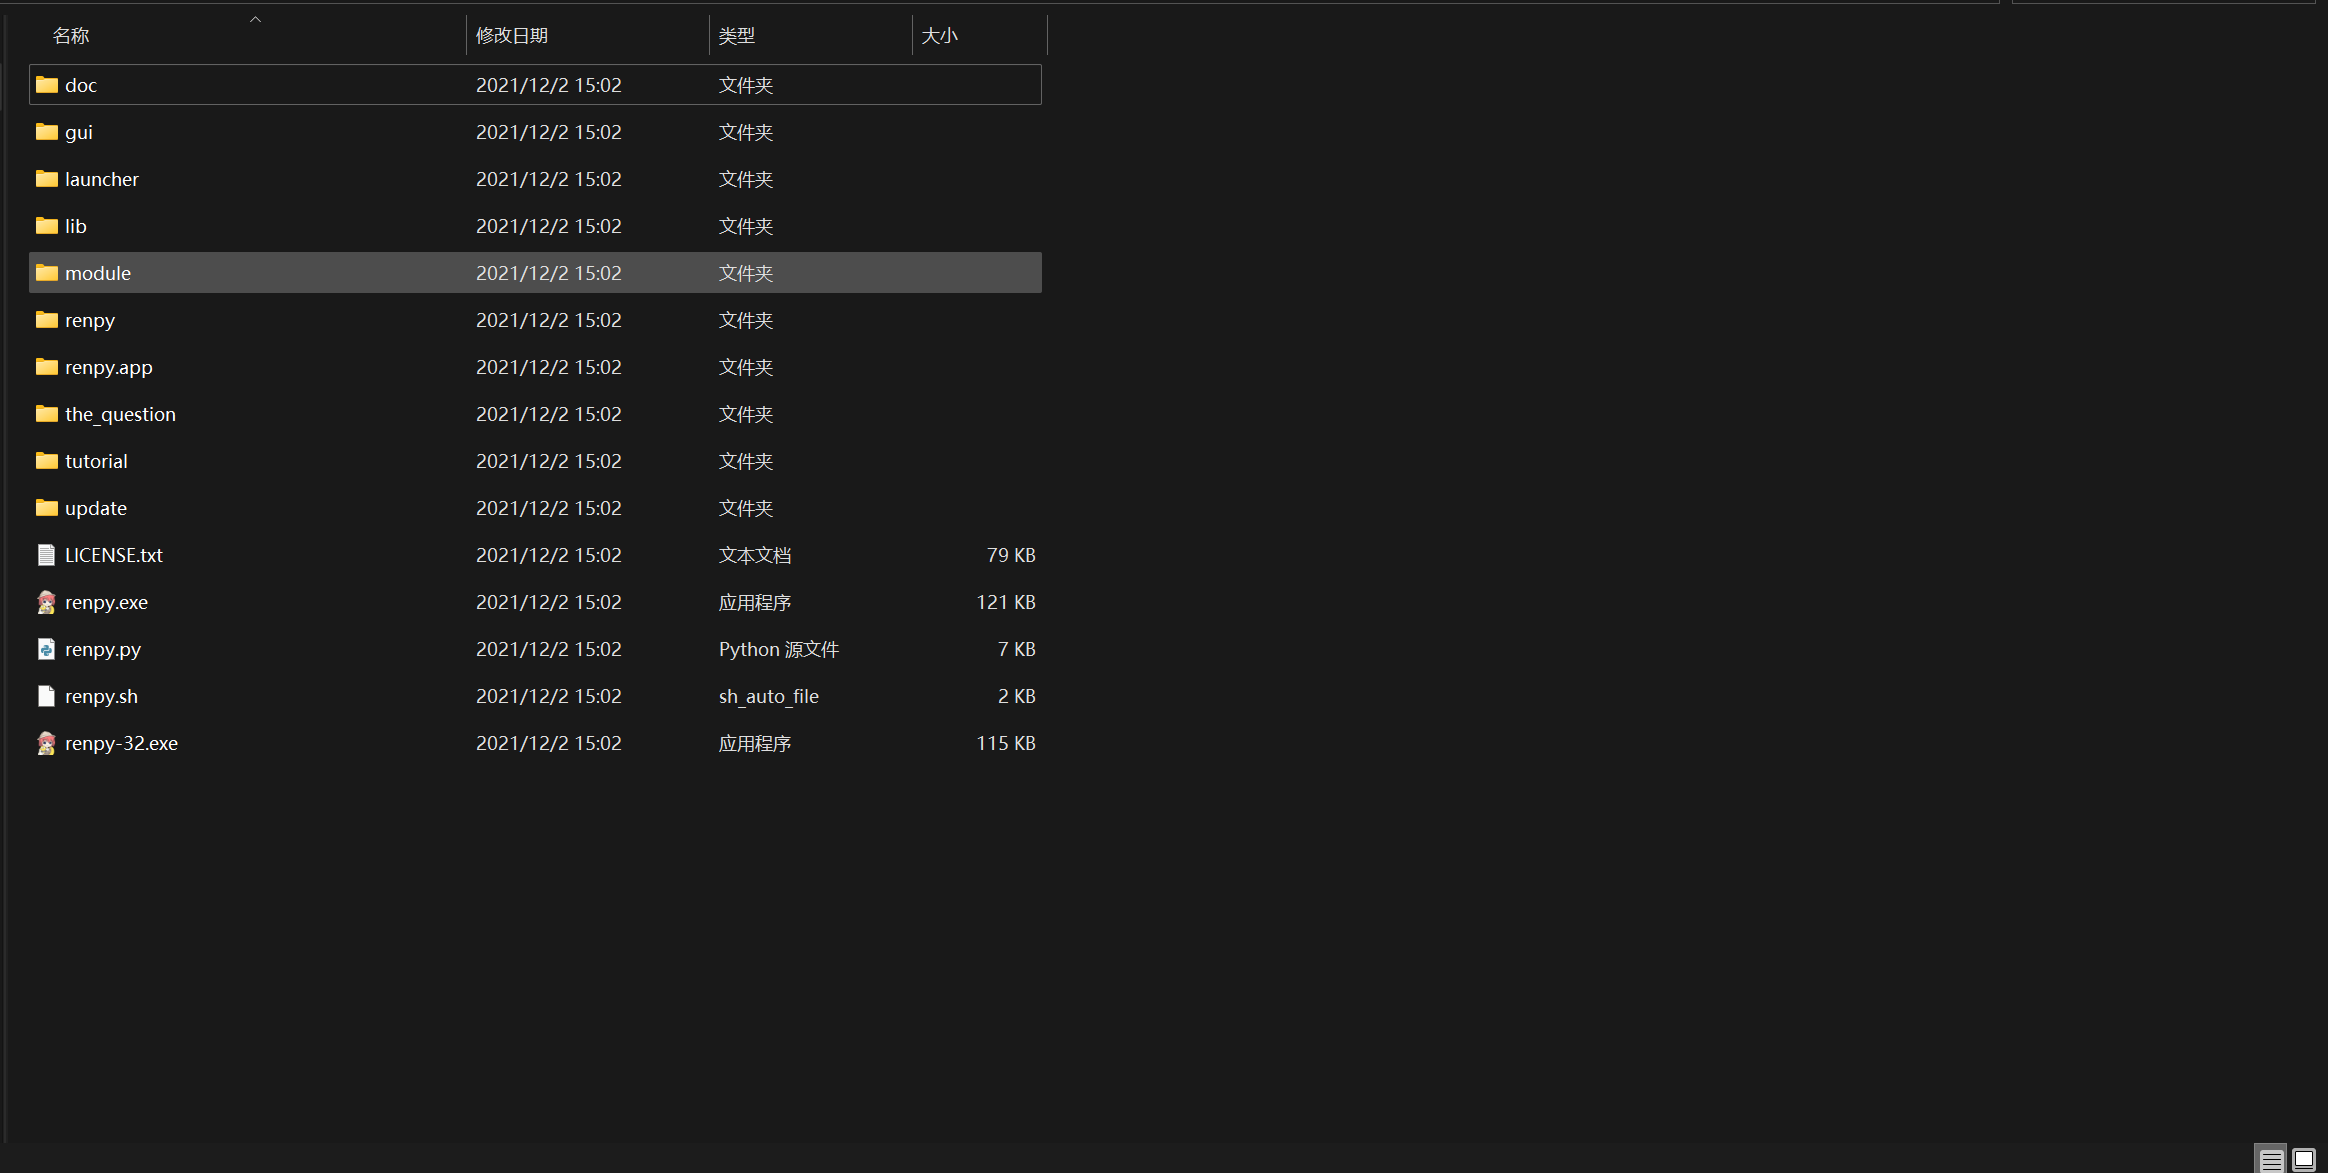
\includegraphics[scale=.15]{Pictures/1/1.2/1.2.3.png}
        \caption{文件夹内容}
        \label{fig:2.2.3}
    \end{minipage}
\end{figure}
以ZIP文件为例,下载完成后打开压缩包(如图\ref{fig:2.2.2})
将文件夹中的所有内容解压,得到如下内容。(如图\ref{fig:2.2.3})

Windows用户请双击renpy.exe或renpy-32.exe(在某些情况下,它可能显示为renpy或renpy-32);MacOS用户若使用驱动器镜像(dmg)安装Ren'Py,挂载后将renpy-7.6.1复制到桌面,进入桌面上的文件夹并运行renpy。;Linux用户请运行renpy.sh。

\begin{figure}[htbp]
    \centering
    \begin{minipage}{182pt}
        \centering
        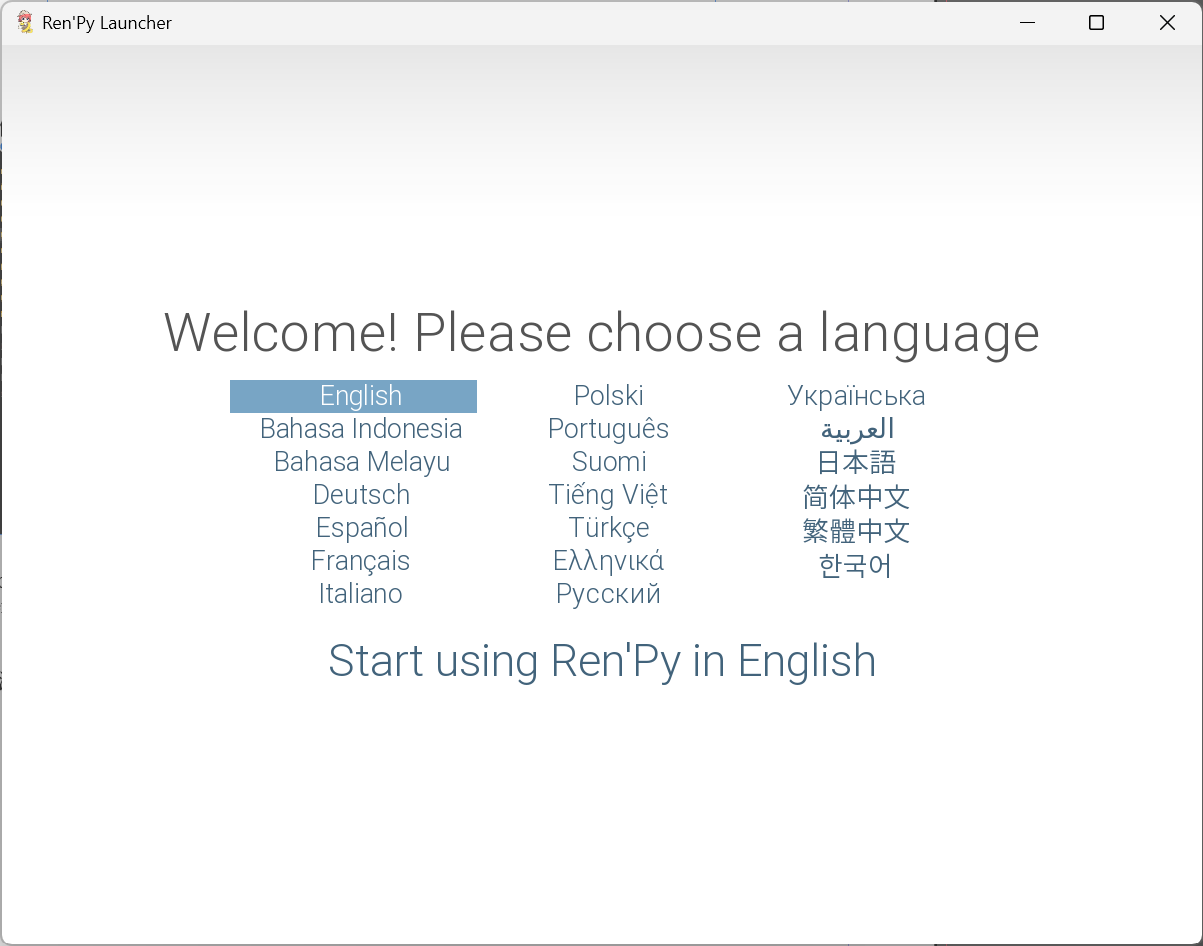
\includegraphics[scale=.2]{Pictures/1/1.2/1.2.4.png}
        \caption{选择语言}
        \label{fig:2.2.4}
    \end{minipage}
    \hspace{10pt}
    \begin{minipage}{182pt}
        \centering
        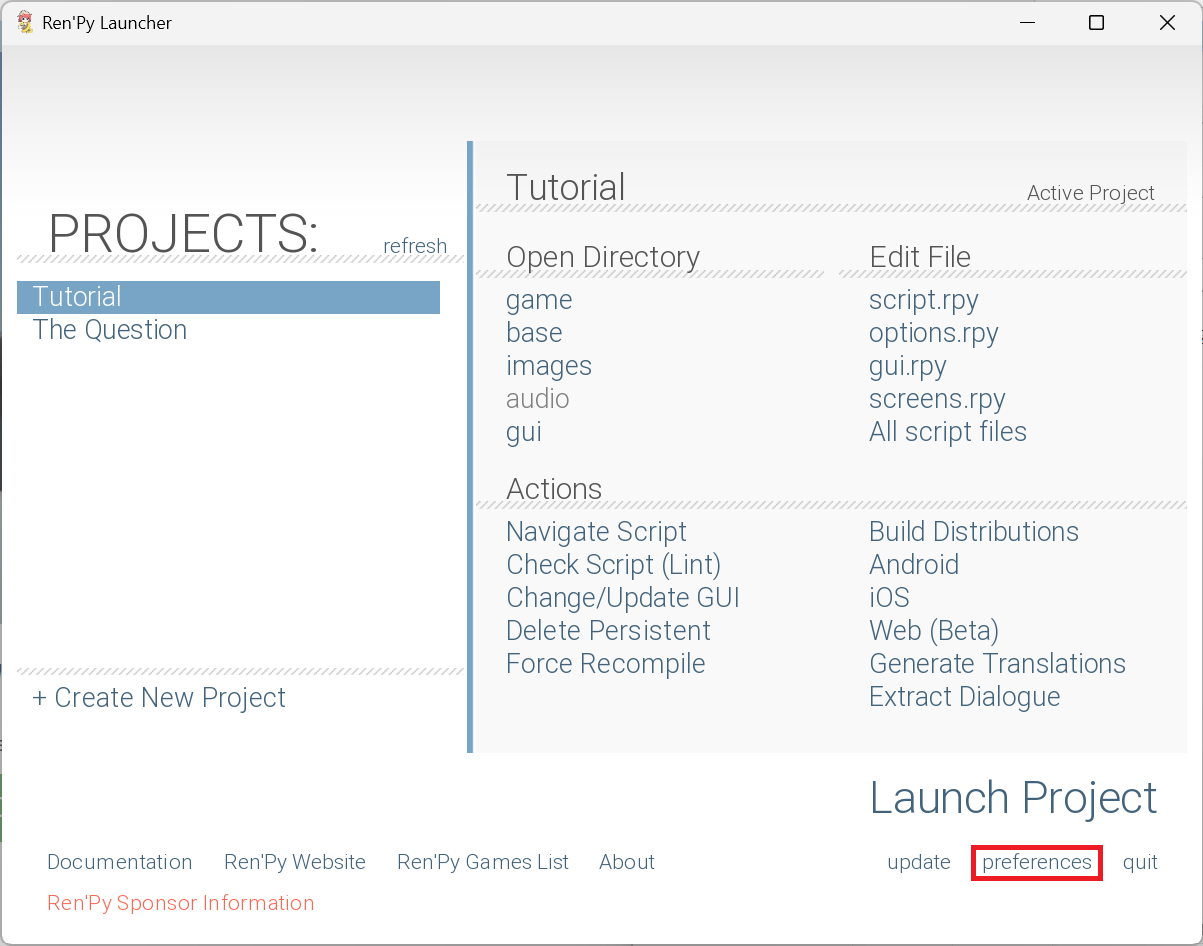
\includegraphics[scale=.2]{Pictures/1/1.2/1.2.5.png}
        \caption{调整语言}
        \label{fig:2.2.5}
    \end{minipage}
\end{figure}

打开Ren'Py后,正常来讲,您会见到如图\ref{fig:2.2.4}所示的界面。点击简体中文后,您会见到如图\ref{fig:2.2.5}所示的界面。

若您没有见到该界面,而是直接见到类似图\ref{fig:2.2.5},请点击右下角的preferences,在右下角Language中选中简体中文即可调整为简体中文。

\chapter{开始学习Ren'Py}

\begin{ChapterGoals}
    \begin{itemize}
        \item \FZFangSong 使用DDLC Mod中文模版创造一个项目;
        \item \FZFangSong 学会使用say语句;
        \item \FZFangSong 学会使用show、hide、scene语句;
        \item \FZFangSong 学会使用play、stop语句;
        \item \FZFangSong 学会使用menu语句;
    \end{itemize}
\end{ChapterGoals}

要建造一个属于我们的房屋,就必须要先打地基、搭框架。如果说Ren'Py是项目的地基,那么Mod模板就是一个框架,我们可以在这个框架中快速地放置门、窗等,还可以自定义这个框架,而不必先调制水泥,然后从地基一步步开始。通过模版,我们可以省去很多步骤。本章我们将在DDLC Mod中文模版的基础上将对Ren'Py进行初步学习。

\section{准备开发环境}
DDLC Mod模板是由GanstaKingofSA编写的一个方便开发Mod的模板。imgradeone对其进行了本土化。目前,DDLC Mod中文模板主要流行三个大版本:1.0版本,2.0版本(即Next分支)与4.0版本(即Future分支)。
\begin{itemize}
    \item 1.0 版本仅支持 Ren'Py 6,且没有什么特别功能;
    \item 2.0 版本增加支持了 Ren'Py 7、Android 移植等功能;
    \item 4.0 版本增加支持了 Ren'Py 8 与 Python 3,增加额外屏幕(Extra Screen)功能等,但稳定性存疑。
\end{itemize}

本书将使用 2.0 版本进行讲解。

\subsection{下载DDLC Mod中文模版}

\begin{figure}[htb]
    \centering
    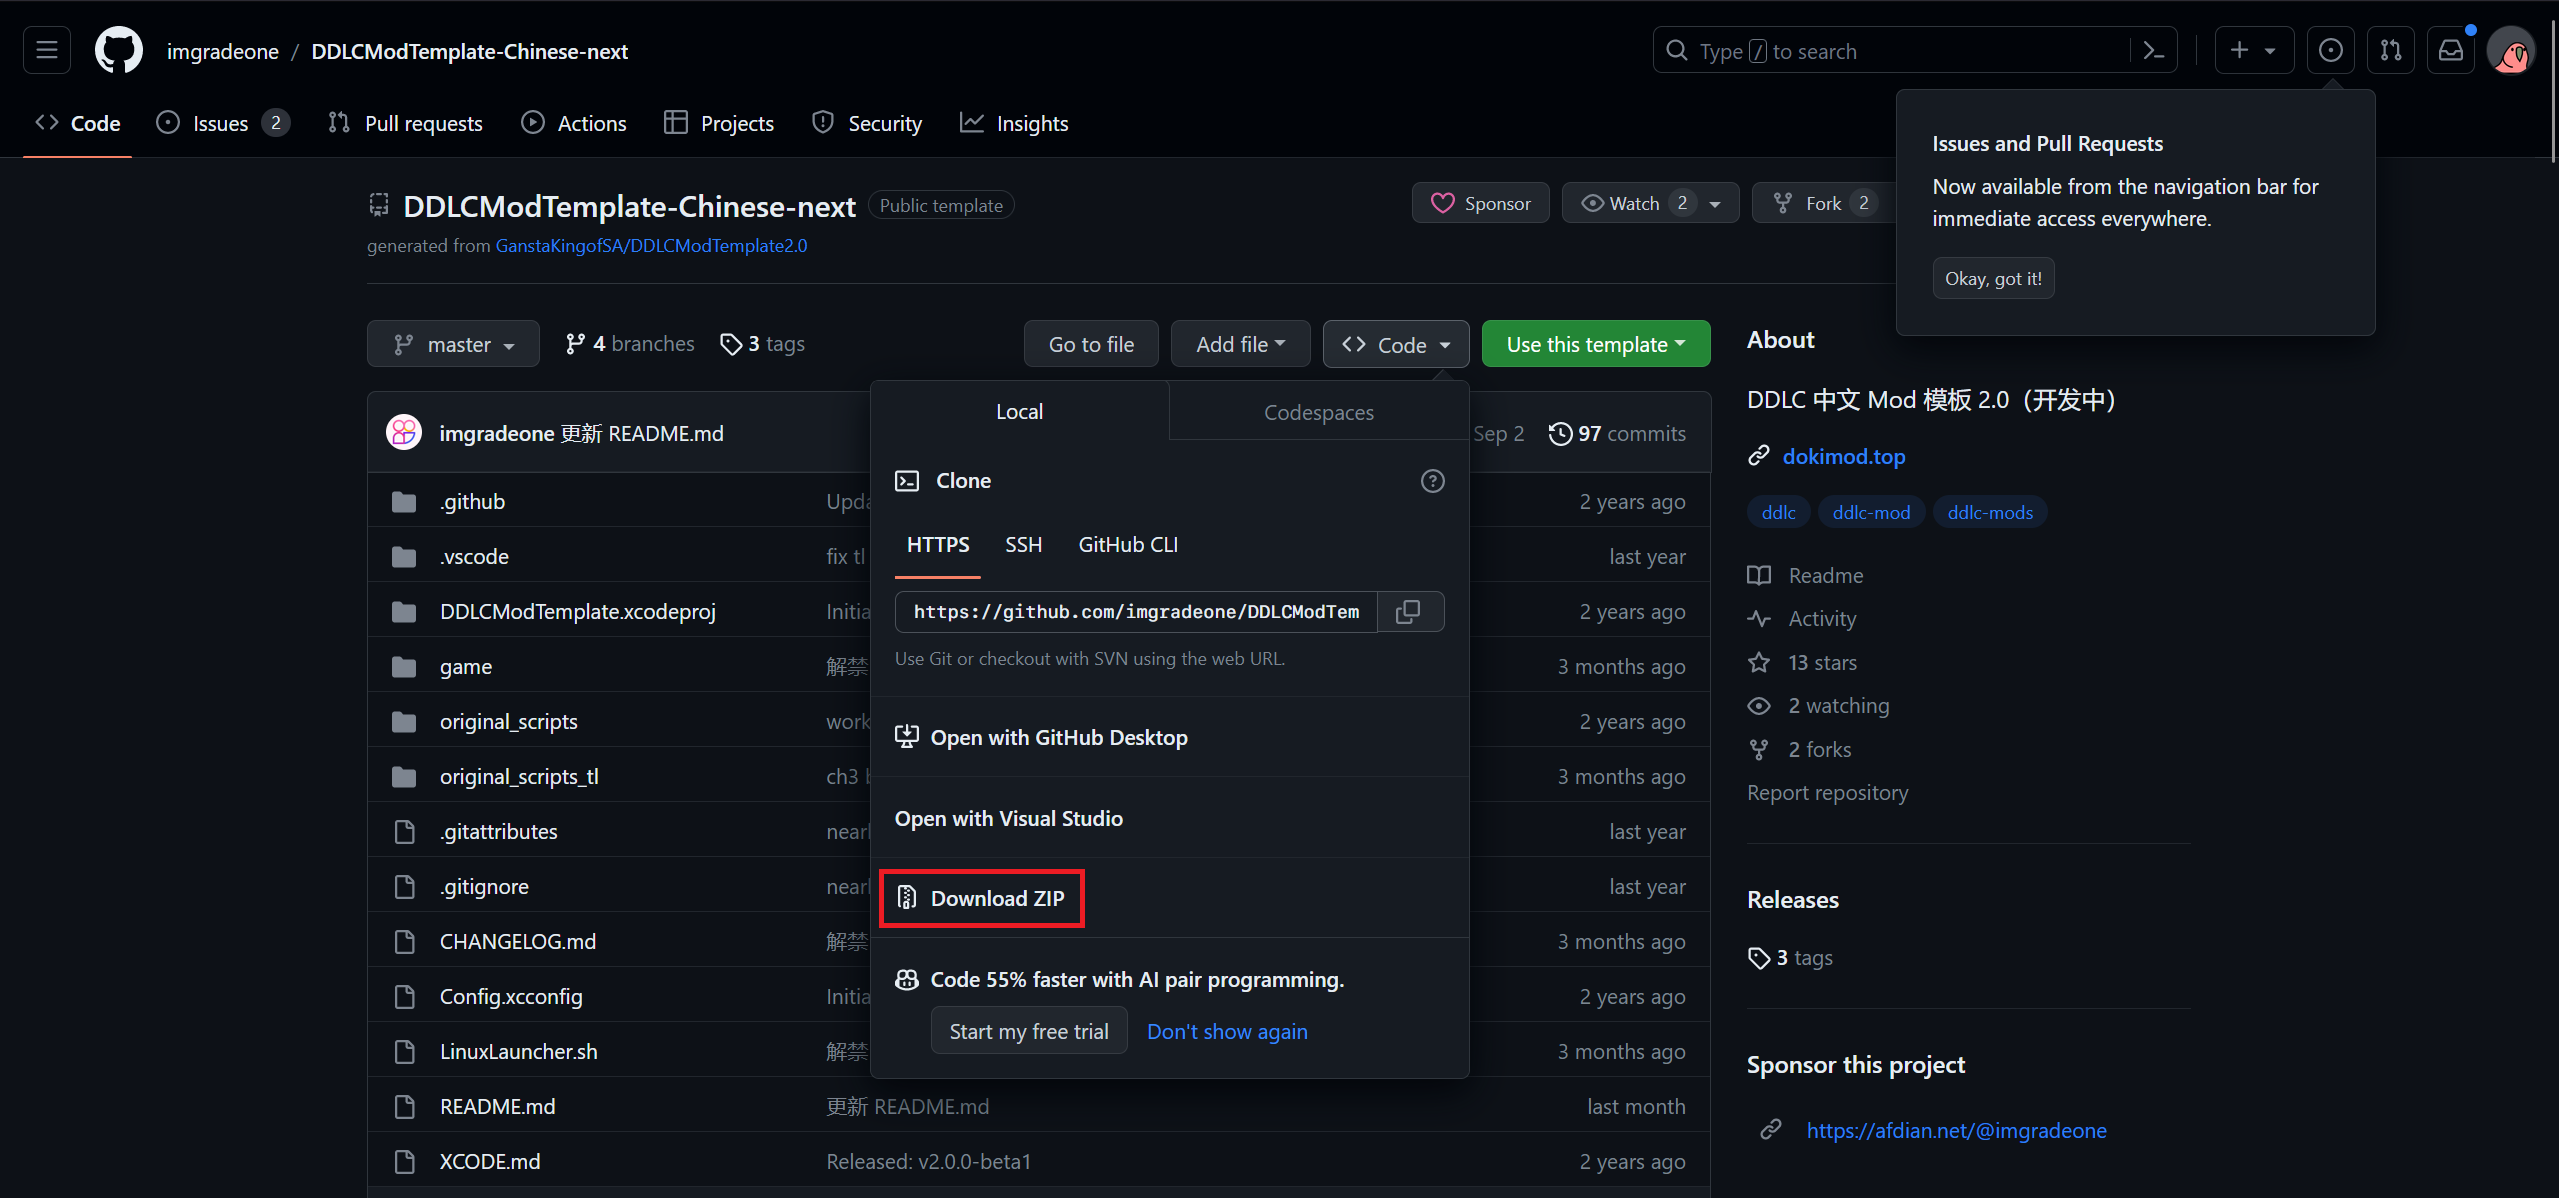
\includegraphics[scale=.15]{Pictures/2/2.1/2.1.1}
    \caption{项目页面}
    \label{fig:3.1.1.1}
\end{figure}
使用任意浏览器打开github.com/imgradeone/DDLCModTemplate-Chinese-next,将压缩包下载下来(如图\ref{fig:3.1.1.1}所示)。

下载完成后解压至在第\ref{sec:2.2.1}节中您下载的Ren'Py SDK的目录下。完成该步骤后,您的Ren'Py SDK中项目一栏应出现DDLCModTemplate-Chinese-next。

从 https://ddlc.moe/中下载原版DDLC,打开压缩包后将DDLC-1.1.1-pc/game/下的audio.rpa、images.rpa、fonts.rpa解压至Mod中文模板下的game/文件夹中。此时,Mod中文模板下的game/文件夹结构应如图\ref{fig:3.1.1.2}所示。

\begin{figure}[htbp]
    \centering
    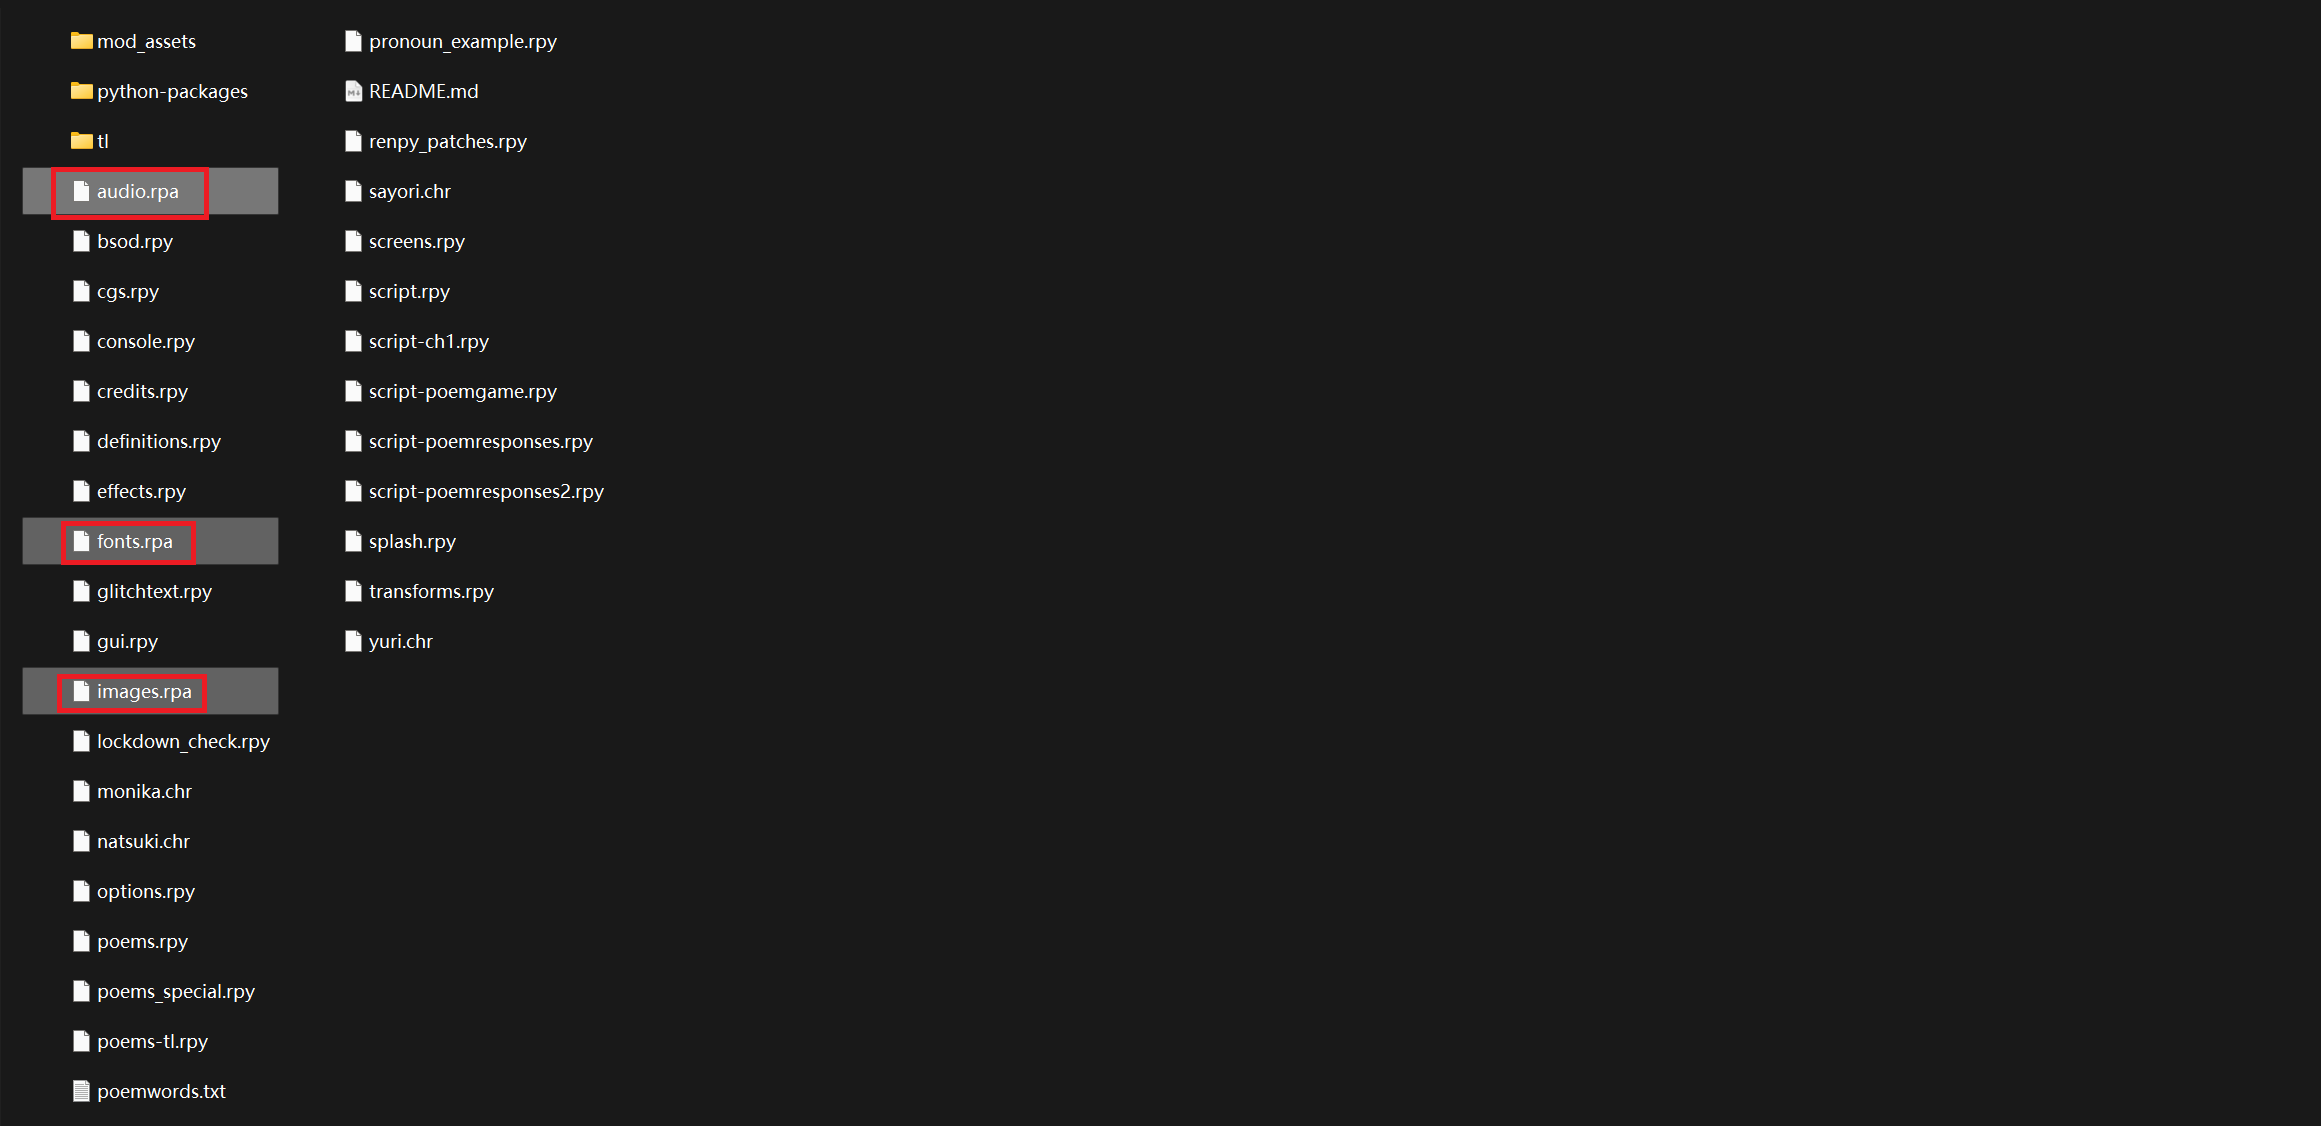
\includegraphics[scale=.2]{Pictures/2/2.1/2.1.2}
    \caption{项目结构}
    \label{fig:3.1.1.2}
\end{figure}

至此,您就完成了准备工作的第一部分———下载DDLC Mod中文模板并完成配置。

\subsection{配置文本编辑器}
有了Mod中文模板,我们还需要一个趁手的编辑器。你大可选择记事本,不过Ren'Py SDK也为我们提供了两种文本编辑器:Visual Studio Code和Atom。本书将以Visual Studio Code为例配置文本编辑器。

打开Ren'Py SDK,点击右下角的设置。在一般选项卡中选择文本编辑器,此时点击第一个选项Visual Studio Code。Ren'Py会开始下载Visual Studio Code与Ren'Py插件。耐心等待一段时间后,会返回到设置界面。此时点击返回,点击DDLCModTemplate-Chinese-next,点击编辑选项卡下的“打开项目”会打开Visual Studio Code(如图\ref{fig:3.1.2.1}所示)。

\begin{figure}[htbp]
    \centering
    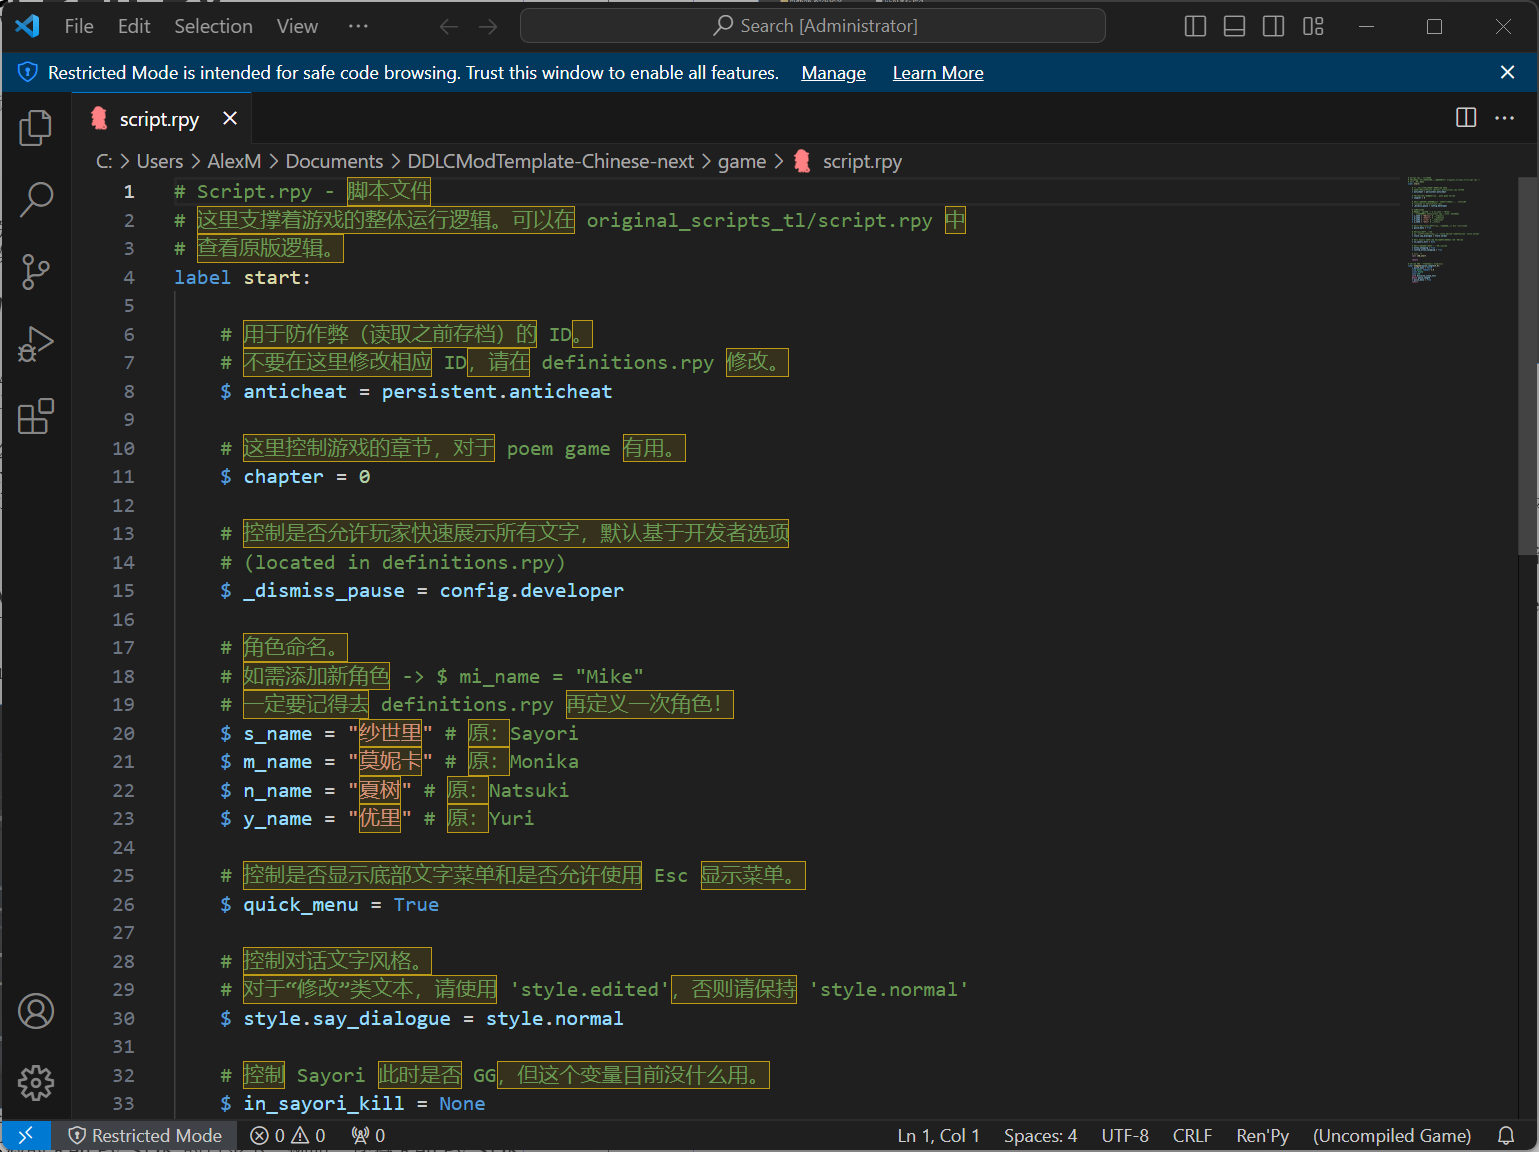
\includegraphics[scale=.4]{Pictures/2/2.1/2.1.3}
    \caption{Visual Studio Code}
    \label{fig:3.1.2.1}
\end{figure}

此时点击扩展选项卡,输入Chinese,点击第一个搜索结果中的Install。此时右下角会弹出提示框询问是否切换语言并重启。点击Change Language and Restart。重启后 Visual Studio Code 就会切换成中文。

打开Ren'Py SDK,选中DDLCModTemplate-Chinese-next,点击编辑文件选项卡中的“打开项目”,Ren'Py SDK会自动帮我们打开Visual Studio Code并定位到本项目。

随后,展开左侧资源管理器中的“game”文件夹,打开script-ch1.rpy文件。保留文件第一行,删除其他内容即可。至此,我们就正式完成了开发的准备工作。

\begin{figure}[htbp]
    \centering
    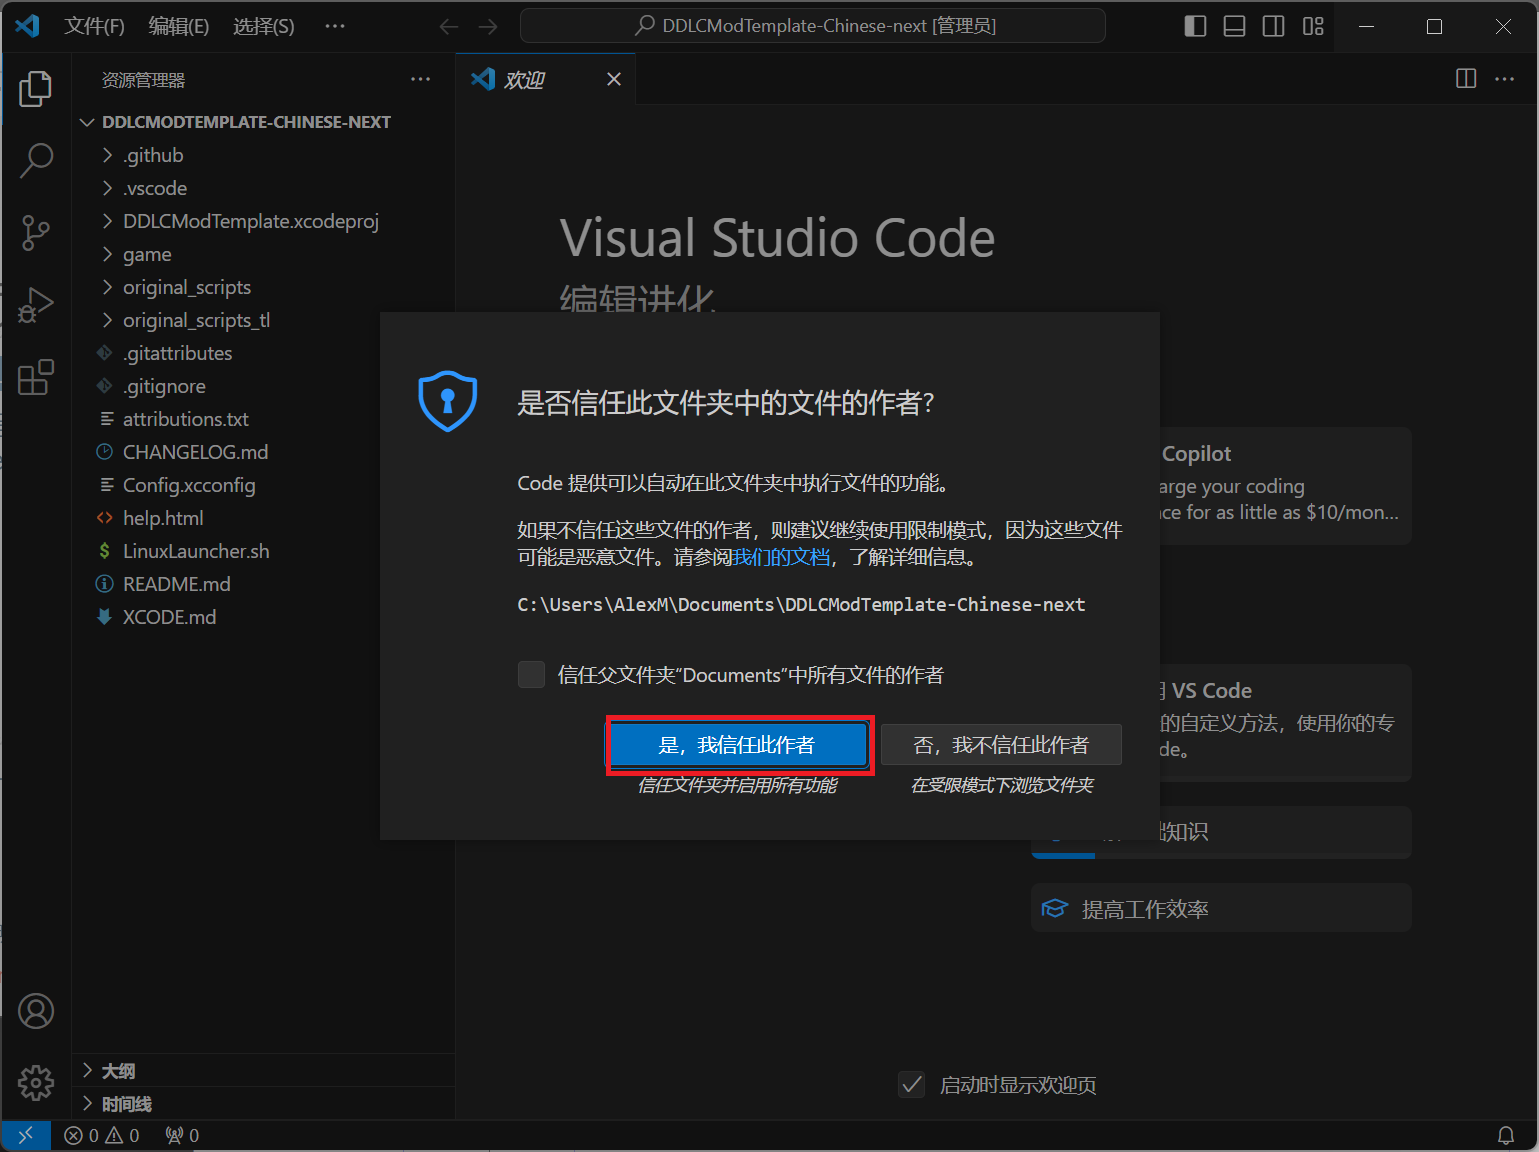
\includegraphics[scale=.4]{Pictures/2/2.2/2.2.1}
    \caption{Visual Studio Code}
    \label{fig:3.1.2.2}
\end{figure}

\begin{Comment}
    若您打开 Visual Studio Code 时出现如图\ref{fig:3.1.2.2}所示的提示框,请点击“是,我信任此作者”。
\end{Comment}

\subsection{设置您的游戏}
做好了上述准备工作,我们还有最后一项任务需要完成————配置你的游戏设置。游戏设置关系到游戏的正常运行、存读档。现在,在Visual Studio Code左侧资源管理器中game目录下的options.rpy文件

现在,将根据下表,将原有内容替换或进行配置。




\section{进入Ren'Py世界}
在Ren'Py的世界里,剧本与视觉内容都围绕着代码展开。要编写脚本,我们就必须先学习Ren'Py的语法。
\subsection{say语句}\label{subsec:3.2.1}
say语句是一个十分重要的语法,它可以让视觉小说角色拥有对话的能力。不过不用担心,say
语句的语法十分简单。

还记得上一课我们打开的script-ch1.rpy吗?现在另起一行,按下 Tab 键(或打四个空格,不过Visual Studio Code会自动为我们将Tab转化为空格),输入以下代码片段:

\begin{lstlisting}
    "快到学园祭了"
    m "各位!我们得开始准备了!"
\end{lstlisting}

\begin{Warning}
您必须使用英文引号来包住文字。另外,请务必注意缩进问题,错误的缩进将会导致代码运行失败。
\end{Warning}

这是一段非常简单的Ren'Py代码,它只包含文字,不显示任何图像或播放任何音效。现在,切换回Ren'Py SDK,点击启动项目,开始游戏,您应该会看到一行旁白以及莫妮卡的一行对话。

在理解以上基础内容之后,我们可以添加更多对话。不过在那之前,你得先了解 say 语句的基础语法:

\begin{lstlisting}[numbers=none]
<角色名> "<说话内容>"
\end{lstlisting}


此处的角色名应对应下列表格:

\begin{center}
    \tablehead{
    \hline
    角色名 & 对应角色 \\
    \hline
    }
    \tabletail{\hline}
    \tablelasttail{\hline}
    \begin{supertabular}{|c|c|}
        \hline
        m & 莫妮卡(Monika)\\
        s & 纱世里(Sayori)\\
        y & 优里(Yuri)\\
        n & 夏树(Natsuki)\\
        mc & 主人公(Main Character)\\
        留空 & 旁白(Narrator)\\
        \hline
    \end{supertabular}
    \captionof{table}{角色名表格}
\end{center}

现在,尝试理解下列代码并运行:

\begin{lstlisting}[caption=scipt-ch1.rpy, label={lst:2.1}]
# Chapter 0
label ch0_start:
    "快到学园祭了。"
    m "各位!我们得开始准备了! "
    s "好耶!!!! "
    n "啊,我都等不及学园祭了。"
    n "肯定会很棒的! "
    y "..."
    return
\end{lstlisting}

在Ren'Py中,我们使用脚本标签(label)来声明代码块。(关于脚本标签的知识,我们将会在后续内容进行详细讲解)。通常,在Ren'Py项目中都含有一个名为start的脚本标签。但是在DDLC Mod 模板中,script.rpy文件已经为我们声明好了start脚本标签。在本段代码中,script-ch1.rpy包含以下几件事:

\begin{itemize}
    \item 第一行的注释;
    \item 创造一个名为ch0\_start的代码块;
    \item say语句创造对话;
    \item return语句返回到上级。
\end{itemize}

\begin{Comment}
在Ren'Py中,我们使用与Python相同的“\#”来表示本行为注释。注释行的内容将不会被 Ren'Py或Python执行。
\end{Comment}

当我们需要在对话中提及玩家的名字、需要将某些内容突出显示或对某部分文字需要进行特殊处理时,应当怎么办呢?读代码\ref{lst:2.2},尝试理解其用法,并在游戏中运行,看看与自己的猜测是否相同。

\begin{lstlisting}[caption=scipt-ch1.rpy, label={lst:2.2}]
# Chapter 0
label ch0_start:
    "{cps=20} 快到 {b} 学园祭 {/b} 了。{/cps}{w=.5}{nw}"
    m "各位!我们得开始准备了!"
    s "好耶!!!!"
    n "啊,我都等不及学园祭了。"
    n "肯定会很棒的!"
    y "..."
    m "那么,是时候来进行分工了。"
    m "[player],你想要做什么?"
    return
\end{lstlisting}

\begin{ExtraKnowledge}
player是一个记录了玩家名字的变量。不理解变量是什么?没关系,本书将在后面为您介绍变量的性质与作用。在这里,您只需要知道当需要提及玩家名字时使用player变量即可。

您或许也注意到了\{/cps\}和\{/b\}。这是对前面cps标签和bold标签的闭合,代表着其适用范围仅为自身标签与闭合标签内的所有文字。
\end{ExtraKnowledge}

不难发现,当需要使用变量时,我们只需要使用中括号将变量名括住。当我们需要将某段文字进行加粗等操作,可以对文字打上标签(既花括号)。若需要在对话中使用这些字符,则需要连续出现两次。如在代码中要出现花括号,则应该使用\{\{\}\}代替\{\}

以下为常用的文字标签:
\begin{center}
    \tablehead{
    \hline
    标签 & 作用\\
    \hline
    }
    \tabletail{\hline}
    \tablelasttail{\hline}
    \begin{supertabular}{|c|c|}
        \hline
        \{b\} & 将文本渲染为粗体 \\
        \hline
        \{i\} & 将文本渲染为斜体 \\
        \hline
        \{color=<16进制颜色>\} & 将文本渲染为指定颜色 \\
        \hline
        \{font=<字体文件>\} & 使用指定字体渲染文本 \\
        \hline
        \{cps=<数字>\} & 以指定速度渲染文本 \\
        \hline
        \{nw\} & 不等待用户操作,渲染完本行文字后立即渲染下一行 \\
        \hline
        \{w=<数字>\} & 等待一定秒数后或用户操作后继续渲染文本 \\
        \hline
    \end{supertabular}
    \captionof{table}{常用文本处理标签}
    \label{table:3.2.1}
\end{center}

\subsection{show、hide、scene语句}

在\ref{subsec:3.2.1}课中,我们学习了如何在视觉小说中编写对话。但现在有一个很大的问题⸺没有图像。在视觉小说中,视觉便是重点。在本课中,我们将学习如何在视角小说中显示图像。

\subsubsection{show语句}

show语句是Ren'Py游戏中的一个重要语句。它可以让一个图像显示在屏幕上。这个图像可以是背景,也可以是角色。

还记得上一课中的代码吗?请阅读以下代码并尝试理解,在Ren'Py中运行,看看运行实际效果与自己的理解是否正确。

\begin{lstlisting}[caption=script-ch1.rpy, label={lst:2.3}]
# Chapter 0
label ch0_start:
    show bg club_day
    "{cps=20}快到{b}学园祭{/b}了。{/cps}{w=.5}{nw}"
    show monika 1a at t41 zorder 1
    m "各位!我们得开始准备了!"
    show sayori 1a at t42 zorder 1
    s "好耶!!!!"
    show natsuki 1a at t43 zorder 1
    n "啊,我都等不及学园祭了。"
    n "肯定会很棒的!"
    show yuri 1a at t44 zorder 1
    y "..."
    m "那么,是时候来进行分工了。"
    m "[player],你想要做什么?"
    return
\end{lstlisting}

由此可知,show语句的基础语法为:
\begin{lstlisting}[numbers=none]
show <图片名称> <附加参数>
\end{lstlisting}

在游戏中,图片名称可以大致分为三类:
\begin{itemize}
    \item 角色立绘
    \item 背景立绘
    \item 毛刺(Glitch)立绘
\end{itemize}

\paragraph{角色立绘}\label{para:3.2.2.1}

对于角色立绘,图片名称的组成为:
\begin{lstlisting}[numbers=none]
<角色名> <立绘编号>
\end{lstlisting}

DDLC原版中,一个显示在屏幕上的角色立绘可以分为两个部分:身体姿势与面部表情。(实际上,DDLC中的立绘为三个部分:左侧身体姿势、右侧身体姿势、面部表情)

模版中已经将所有可能的身体姿势为我们组合好了。除优里外的所有角色都有五个姿势(1-4为正常站位,5为特殊站位),而优里只有4个姿势(1-3为正常站位,4为特殊站位)。

面部表情使用英文小写字母来表示(请注意,不是所有的角色的面部表情都表示到z。如莫妮卡的面部表情就远少于夏树的面部表情)。

同时,除莫妮卡外的所有角色都可以使用日常服,只需要在身体姿势后加上b即可使用日常服。如:1b

对于角色立绘的列举,您可以前往 \url{https://docs.dokimod.top/pages/0a59cf/} 与 \url{https://ddlc-modding.fandom.com/wiki/Expressions_and_Poses} 查看。


\paragraph{毛刺立绘}

毛刺立绘则是指在二周目出现的大多数“错误”立绘,如错乱的莫妮卡等。
对于毛刺立绘,其图片名称的构成为:
\begin{lstlisting}[numbers=none]
<角色名> <毛刺编号>
\end{lstlisting}

\begin{Warning}
    我们不建议您使用毛刺立绘,因为这对于某些厨可能极不友好。
\end{Warning}

一般来说,毛刺编号为glitch。但是请注意,莫妮卡的毛刺立绘编号为g1与g2;夏树的毛刺立绘则包括ghost\_blood、ghost1、ghost2等。

若要使用优里的自杀立绘,则毛刺编号为stab\_+数字1-6。

\paragraph{背景立绘}

对于背景立绘,其图片名称构成为:
\begin{lstlisting}
bg <背景编号>
\end{lstlisting}

背景编号即意义可以在definitions.rpy文件中找到。这里不再进行过多叙述。

\begin{ExtraKnowledge}
通常我们不使用show来显示背景,而是使用scene。对于scene的详细介绍请看第\ref{subsubsec:3.2.2.3}课。
\end{ExtraKnowledge}

\paragraph{附加参数}

对于附加参数,常用的有:
\begin{center}
    \tablehead{
    \hline
    语法 & 作用\\
    \hline
    }
    \tabletail{\hline}
    \tablelasttail{\hline}
    \begin{supertabular}{|c|c|}
        \hline
        at <transform> & 将一个动画(transform)套用到立绘上\\
        \hline
        with <transform> & 显示图像时使用指定的转场动画(transform)\\
        \hline
        zordr <数字> & 控制图像在Z轴上的位置\\
        \hline
    \end{supertabular}
    \captionof{table}{常用show语句附加参数}
\end{center}

\begin{ExtraKnowledge}
show语句也可以使用behind 从句、as从句、onlayer从句。但由于在游戏中这些从句很少会使用,故不再展开讲解。有兴趣者可前往 \url{https://doc.renpy.cn/zh-CN/displaying_images.html} 了解详细内容。
\end{ExtraKnowledge}

\subparagraph{at、with从句}
\label{subsubsec:3.2.2.1}
当变换作为角色动画时,应使用at从句。一个关于变换的例子:t41。在这个变换中,t表示在这个位置上的角色静止站立在原地;4表示一共有4个站位,会将屏幕等分成4份;1表示从左往右该变换是所有站位中的第1个。

所有角色状态有:

\begin{center}
    \tablehead{
    \hline
    编号 & 意义\\
    \hline
    }
    \tabletail{\hline}
    \tablelasttail{\hline}
    \begin{supertabular}{|c|c|}
        \hline
        t & 角色静止站立在原地 \\
        \hline
        i(instant) & 角色突然出现 \\
        \hline
        f(focus) & 角色成为屏幕焦点 \\
        \hline
        s(sink) & 角色下沉 \\
        \hline
        h(hop) & 角色跳跃 \\
        \hline
        hf(hop and focus) & 角色跳跃并成为屏幕焦点 \\
        \hline
        d(dip) & 角色向下倾斜然后升起 \\
        \hline
        l(left) & 角色从左侧飞入 \\
        \hline
        r(right) & 角色从右处飞入 \\
        \hline
    \end{supertabular}
    \captionof{table}{角色状态表}
\end{center}


对于站位总数,共有1到4。

当变换作为转场动画来使用时,应使用with从句。游戏中实现定义好的转场动画有:

\begin{center}
    \tablehead{
    \hline
    编号 & 意义\\
    \hline
    }
    \tabletail{\hline}
    \tablelasttail{\hline}
    \begin{supertabular}{|c|c|}
        \hline
        dissolve & 溶解效果 \\
        \hline
        dissolve\_cg & 适用于CG的溶解效果 \\
        \hline
        dissolve\_scene & 适用于scene的溶解效果 \\
        \hline
        dissolve\_scene\_full & 使屏幕自行溶解为黑色,显示另一个场景 \\
        \hline
        dissolve\_scene\_half & 溶解屏幕一段时间,显示下一个场景 \\
        \hline
        wipeleft & 从屏幕左侧擦除隐藏当前图像 \\
        \hline
        wipeleft\_scene & 从屏幕左侧擦除屏幕为黑色,然后显示下一场景 \\
        \hline
        wiperight & 从屏幕右侧擦除隐藏当前图像 \\
        \hline
        wiperight\_scene & 从屏幕右侧擦除屏幕为黑色,然后显示下一场景 \\
        \hline
    \end{supertabular}
    \captionof{table}{常用转场动画编号及其效果}
\end{center}


\subparagraph{zorder从句}
对于zorder从句,zorder后的数字越大,图像在Z轴上的距离越远,即离屏幕越远,反之亦然。但由于DDLC的变换已经为我们设置好了图像的大小,所以zorder其实在后续版本不再需要。

\paragraph{临时性变化与对话属性}
在视觉小说中,每一次对话角色的神态、姿势可能都会发生变化,那我们岂不是要重复使用很多次show语句、hide语句?所以为了方便开发,Ren'Py给say语句添加了对话属性。

如下例:
\begin{lstlisting}
# Chapter 0
label ch0_start:
    show bg club_day
    "{cps=20}快到{b}学园祭{/b}了。{/cps}{w=.5}{nw}"
    show monika 1a at t41 zorder 1
    m "各位!我们得开始准备了!"
    show sayori 1a at t42 zorder 1
    s "好耶!!!!"
    show natsuki 1a at t43 zorder 1
    n 2d "啊,我都等不及学园祭了。"
    n "肯定会很棒的!"
    show yuri 1a at t44 zorder 1
    y "..."
    m "那么,是时候来进行分工了。"
    m 4k "[player],你想要做什么?"
    return
\end{lstlisting}

运行后,我们发现,当夏树说出“啊,我都等不及学园祭了。”会变换一次立绘,以及后面莫妮卡说出“[player],你想要做什么?”也会变换立绘,这就是say语句的对话属性作用。

不难发现,只需要在角色名后添加立绘编号即可使角色在说出这句话时变换为指定立绘。

临时性变化则是指角色在说出本句前会变换为指定立绘,在本句结束后则换回原来的立绘。要启用临时性变化,只需要在角色名后的立绘编号前加上@即可。如:
\begin{lstlisting}[numbers=none]
    n @2d "啊,我都等不及学园祭了。"
\end{lstlisting}

\subsubsection{hide语句}

hide语句有着与show语句相反的作用⸺从屏幕上隐藏一个图像。如:

\begin{lstlisting}[numbers=none]
hide monika
\end{lstlisting}

则会将莫妮卡从当前屏幕上隐藏。

hide语句同样可以使用附加参数,但只能使用with从句,使用方法与show语句的with从句相同,详细请见第\ref{subsubsec:3.2.2.1}课。

\begin{ExtraKnowledge}
    扩展知识:hide语句同样可以使用onlayer从句,用于隐藏对应图层上的图像。但在游戏中很少会涉及到对图层的操作,故本书不会对onlayer从句展开讲解。有兴趣者课前往 \url{https://doc.renpy.cn/zh-CN/displaying_images.html} 了解详细内容。
\end{ExtraKnowledge}

\subsubsection{scene语句}
\label{subsubsec:3.2.2.3}

scene语句类似于show语句,但与show语句有一个很明显的差异⸺使用scene语句会清空当前屏幕上的所有图像。scene语句的显示方式和特性的使用效果与show语句一致。

尝试在游戏中运行以下代码,并猜测运行结果:
\begin{lstlisting}[caption=script-ch1.rpy]
# Chapter 0
label ch0_start:
    scene bg club_day
    "{cps=20}快到{b}学园祭{/b}了。{/cps}{w=.5}{nw}"
    show monika 1a at l41 zorder 1
    m "各位!我们得开始准备了!"
    show sayori 1a at h42 zorder 1
    s "好耶!!!!"
    show natsuki 1a at t43 zorder 1
    n 2d "啊,我都等不及学园祭了。"
    n "肯定会很棒的!"
    show yuri 1a at s44 zorder 1
    y "..."
    scene bg club_day
    show monika 2a at t11 zorder 1
    m "那么,是时候来进行分工了。"
    m 4k "[player],你想要做什么? "
    return
\end{lstlisting}

不难发现,执行scene语句时会将整个屏幕清空。scene语句的语法为:

\begin{lstlisting}[numbers=none]
scene <图片编号> <with从句>
\end{lstlisting}

with从句的使用方法与hide、show语句相同。详细请见\ref{subsubsec:3.2.2.1}。

\subsection{play、stop、voice语句}
现在,在我们的视觉小说中,图像有了,人物立绘与背景也有了,但还是缺了一些东西,比如音
乐与音效。在接下来,我们将会进入对于play和stop语句的学习。

\subsubsection{play语句}

play语句主要用于播放音频、音效。请注意,play语句会覆盖当前通道所播放的音频。

Ren'Py中,我们主要使用三种已经定义好的音频频道:

\begin{itemize}
    \item music - 音乐播放通道;
    \item sound - 声音播放通道;
    \item voice - 语音播放通道。 
\end{itemize}

请阅读以下代码并尝试理解play语句的语法:

\begin{lstlisting}
    play music audio.t1
    play sound audio.closet_open
\end{lstlisting}

不难看出,play语句的基本语法如下:
\begin{lstlisting}[numbers=none]
play <频道名> <文件名>
\end{lstlisting}

\begin{ExtraKnowledge}
    在上述例子中,audio.t1是一个变量,且被定义为"<loop 22.073>bgm/1.ogg"。故此处的文件名也可以是一个指向文件名的变量。
\end{ExtraKnowledge}

对于DDLC中音乐的定义,您可以查阅definitions.rpy中的注释。

\paragraph{播放列表}
play语句的文件名部分也可以是一个列表,且遵循从首到尾的顺序。

读下列代码,尝试理解并运行:
\begin{lstlisting}
    play music [audio.t1, audio.t2]
    play sound [audio.closet_open, "<silence .5>", audio.closet_open]
\end{lstlisting}


\paragraph{特殊效果}
play也可以使用淡出、淡入、循环等效果。

读下列代码,尝试理解并运行。
\begin{lstlisting}
    play music audio.main_menu loop
    play music audio.t1 fadein .5 fadeout 1 noloop
\end{lstlisting}

从实际效果可以看出,loop可以使一段音频重复播放;fadein则可以使音频在指定时间内淡入;fadeout则使音频在指定时间内淡出;noloop意味不重复播放这段音频。

\begin{ExtraKnowledge}
    当play语句既没有出现loop分句也没有出现noloop分句时,Ren'Py会根据音频的默认配置决定音频的播放。
\end{ExtraKnowledge}

play语句同样也可以调整音频的音量。
\begin{lstlisting}[numbers=none]
    play music audio.t1 volume .55 loop
\end{lstlisting}
请注意,volume分句后的值应大于等于0小于等于1

\subsubsection{stop语句}

stop语句以关键词stop开头,后接想要停止播放的通道名。如:
\begin{lstlisting}[]
    stop music fadeout 2
    stop sound
\end{lstlisting}

\subsubsection{voice语句}
Ren'Py同样支持语音功能。要使用语音功能可以使用voice语句。

读下列代码,尝试理解voice语句的用法:
\begin{lstlisting}
    voice 'hello.ogg'
    m "你好!"

    define voice.a = "happy_birthday.ogg"
    voice voice.a
    m "生日快乐!"
\end{lstlisting}

请注意,当用户进行互动行为时,语音将会被打断。使用sustain特性则可以保证语音完整播放不被打断。
\begin{lstlisting}
    voice 'arguing.ogg'
    s "你不能这样做!!"

    voice sustain
    s "...小蛋糕是我的!!!!"
\end{lstlisting}

\paragraph{自动语音}
Ren'Py同时还提供了自动语音功能,省去了麻烦的voice语句。

要实现这个功能,语音文件名必须跟对话脚本标识号严格匹配。

对话脚本标示名,需要将对话脚本导出为一个表格。操作如下:
\begin{enumerate}
    \item 在启动器上选择“Extract Dialogue”
    \item “Tab-delimited Spreadsheet (dialogue.tab)”
    \item “Continue”
    \item 使用表格程序打开dialogue.tab。
\end{enumerate}

表格的第一列就是需要使用的标识号,其他列则是对话的更多别的信息。

要自动播放语音,请将config.auto\_voice设置为一个包含\{id\}的字符串。当开始对话时,\{id\}会被对话脚本标识符替换,并自动组成一个音频文件名。若音频文件名对应的文件真实存在,则那个文件就会播放。

\begin{lstlisting}
    config.auto_voice = "mod_assets/voice/{id}.ogg"
\end{lstlisting}

对话标识号是ch1\_n\_end\_24e41fcf,那么当对应的对话显示时,Ren'Py会寻找文件mod\_asset

s/voice/ch1\_n\_end\_24e41fcf.ogg。如果文件存在,Ren'Py会播放这个文件。

\subsection{menu语句}
在视觉小说中,往往会有很多选择。这些选择通常能够影响剧情的走向,进入不同的分支。在本节中,你将会学习menu语句的基本用法。

读下列代码并尝试运行,看看实际的运行效果:
\begin{lstlisting}[caption=script-ch1.rpy]
# Chapter 0
label ch0_start:
    scene bg club_day
    "{cps=20}快到{b}学园祭{/b}了。{/cps}{w=.5}{nw}"
    show monika 1a at l41 zorder 1
    m "各位!我们得开始准备了!"
    show sayori 1a at h42 zorder 1
    s "好耶!!!!"
    show natsuki 1a at t43 zorder 1
    n 2d "啊,我都等不及学园祭了。"
    n "肯定会很棒的!"
    show yuri 1a at s44 zorder 1
    y "..."
    scene bg club_day
    show monika 2a at t21 zorder 1
    show sayori 2a at t22 zorder 1
    m "那么,是时候来进行分工了。"
    m 4k "[player],你想要做什么? "
    menu:
        "做小蛋糕":
            s "夏树的小蛋糕最好吃了!"
        "布置教室":
            m "那我们可得抓紧时间了!"
    return
\end{lstlisting}

menu的基本语法为:
\begin{lstlisting}
    menu:
        "这是一个选项示例" # 文本框内显示的内容。
        "选项 1": # 选项名称
            # 选择此项后所的脚本。
        # 可以添加更多选项。
\end{lstlisting}

\chapter{Python与Ren'Py}
\begin{ChapterGoals}
    \begin{itemize}
        \item 了解Python的基本数据类型;
        \item 学会使用函数与类;
        \item 学会在Ren'Py代码中嵌入Python代码;
        \item 学会使用变量;
        \item 学会进行判断控制;
        \item 学会使用等效语句;
    \end{itemize}
\end{ChapterGoals}

Ren'Py与Python是一个不可分割的整体,在Ren'Py中,许多复杂的操作都需要依靠Python来完成。本章我们将会初步学习如何在Ren'Py中使用Python语句。

\begin{Attention}
    本章只会浅显的介绍Python的用法,若要真正的学习Python,您可以前往 \url{https://www.runoob.com/python3/python3-tutorial.html} 进行更深入的学习。切记,本书不以Python为主。
\end{Attention}

\begin{Warning}
    如果您只是想要简单开发一个Mod,不需要做什么复杂的处理,如只是扩展一下原作剧情,或是给玩家讲述另一个故事,那么您大概率可以跳过本章关于函数、类的学习。但如果您需要开发更复杂的Mod,比如与DDLC有关的AVG游戏,或是像Monika After Story一样的Mod,那么函数与类无疑会方便您后期的开发。

    但是在学习前,您需要注意一些问题。学习Python的难度也比Ren'Py要大许多。而且在Ren'Py中使用Python代码还要格外小心。如在Python中,有几种数据类型需要格外注意。这些数据类型轻则导致代码出现意料之外的运行结果,重则使Ren'Py不稳定崩溃。

    最后,虽然很多Ren'Py语句都有等效的Python代码,但对于Mod来说,不应该使用Python代替Ren'Py代码。Python的作用是方便开发者进行更复杂的操作而不用修改Ren'Py的底层逻辑。但对于大部分的Mod来说,完全可以使用纯Ren'Py代码。更不用说Python代码在一定程度上会增加脚本的复杂度。Python学好了,用好了,就是锦上添花;如果用不好,就会造成开发难度直线上升,Debug及其困难,还会使游戏崩溃给玩家带来负面体验。
\end{Warning}
\section{Python中的几种数据类型}
\subsection{数字}
在大多数编程语言中,数字可以分为两类——整型(int)与浮点类(float)型。整型顾名思义,就是指3、2、6、-2等不包含小数的数字,浮点型则与之相反,即包含小数的数字,如-2.9、7.1、3.213等。

数字可以进行运算,如加减乘除。在Python中,加法运算使用+号,减法运算使用--号,乘法运算使用*号,除法运算使用/号。对于其他的运算符,详细请见表\ref{table:3.1}。如下例:
\begin{lstlisting}
>>> 1 + 2
%\Output{3}%

>>> 2 / 2
%\Output{1.0}%

>>> 10 - 8
%\Output{2}%

>>> 2 * 7
%\Output{14}%
\end{lstlisting}

\begin{ExtraKnowledge}
    我们可以使用变量将想要将数据保存。使用=操作符对变量进行赋值,如:
    \begin{lstlisting}[numbers=none]
>>> a = 1
>>> a
%\Output{1}%

>>> a = a * 2
>>> a
%\Output{2}%
    \end{lstlisting}
\end{ExtraKnowledge}

对于乘方、整除、取模(余数)计算,则分别使用**运算符、//运算符与\%运算符。如下例:
\begin{lstlisting}
>>> 1 ** 2
%\Output{2}%

>>> 2 ** 3
%\Output{8}%

>>> 10 // 8
%\Output{1}%

>>> 14 // 7
%\Output{2}%

>>> 14 %\%% 7
%\Output{0}%

>>> 25 %\%% 4
%\Output{1}%
\end{lstlisting}

\subsection{字符串}
除了数字,Python还可以处理字符串(str)。在Python中可以使用双引号会单引号括起来表示字符串,也可以使用反斜线操作符对特殊字符转义。

\begin{lstlisting}
>>> 'Hello'
%\Output{'Hello'}%

>>> "Hi!"
%\Output{"Hi!"}%

>>> 'I\'m fine.'
%\Output{"I'm fine."}%

>>> "I'm fine."
%\Output{"I'm fine."}%

>>> print("This is a backslash: \\")
%\Output{This is a backslash: \textbackslash}%

\end{lstlisting}

在Python中,字符串同样支持一些运算功能。+号能将两个字符串连接起来。*则用来重复字符串。如:

\begin{lstlisting}
>>> 'Hello! ' * 3
%\Output{'Hello! Hello! Hello!'}%

>>> "Hi! " + "How are you?"
%\Output{"Hi! How are you?"}%

\end{lstlisting}

\begin{center}
    \tablehead{
    \hline
    操作符 & 描述 & 示例 \\
    \hline
    }
    \tabletail{\hline}
    \tablelasttail{\hline}
    \begin{supertabular}{|c|c|c|}
        \hline
        + & 加法运算,将运算符两侧值相加 & 1 + 2; "str" + "string" \\
        \hline
        - & 减法运算,将运算符两侧值相减 & 1 - 2\\
        \hline
        * & 乘法运算,将操作符两侧值相称 & 4 * 2;"str" * 3\\
        \hline
        / & 除法运算,左操作数除以右操作数 & 3 / 1\\
        \hline
        \% & 取模运算,左操作数除以右操作数的余数部分 & 7 \% 2\\
        \hline
        ** & 幂运算,左操作数的右操作数次幂 & 2 ** 3\\
        \hline
        // & 整除运算,左操作数整除以右操作数& 3 // 2\\
        \hline
        += & 将左侧值加上右侧值 & a += 100\\
        \hline
        -= & 将左侧值减去右侧值 & a -= 100\\
        \hline
        *= & 将左侧值乘上右侧值 & a *= 100\\
        \hline
        /= & 将左侧值除以右侧值 & a /= 100\\
        \hline
    \end{supertabular}
    \captionof{table}{常见算数与赋值运算符与示意}
    \label{table:3.1}
\end{center}


\subsection{列表与元组}

\subsubsection{列表}

在Python中,列表(list)是一种常见的数据类型。在列表可以将多种数据组合在一起。如:
\begin{lstlisting}
>>> ['1', '2', '3']
%\Output{['1', '2', '3']}%

>>> ['This', 'is', 'a', 'list']
%\Output{['This', 'is', 'a', 'list']}%

\end{lstlisting}


在列表中,我们可以使用索引(index)来访问指定数据。如:
\begin{lstlisting}
>>> name_list = ['Sayori', '莫妮卡', 'Yuri', 'Natsuki']
>>> name_list[0]
%\Output{'Sayori'}%

>>> name_list[3]
%\Output{'Natsuki'}%
\end{lstlisting}

\begin{Warning}
    从上例中,我们可以知道索引从0开始。但请注意:索引最大值不可以超出列表的长度。即在name\_list这个列表中,索引最大只能为3,因为此时从0往后数4个数为3。如果索引最大值超出了列表长度,Python就会抛出IndexError错误。如:
    \begin{lstlisting}[numbers=none]
>>> name_list = ['Sayori', 'Monika']
>>> name_list[2]

Traceback (most recent call last):
  File "<stdin>", line 1, in <module>
IndexError: list index out of range
    \end{lstlisting}
\end{Warning}

\begin{ExtraKnowledge}
    索引的值也可以为负数,此时Python会从列表尾部向前寻找索引。但请注意,若要使Python从尾部开始寻找,则索引从-1开始,且同样不可超出列表最大长度。如下例:
    \begin{lstlisting}[numbers=none]
>>> name_list = ['Sayori', 'Monika', 'Natsuki', 'Yuri']
>>> name_list[-1]
%\Output{'Yuri'}%

>>> name_list[-4]
%\Output{'Sayori'}%

>>> name_list[-10]
Traceback (most recent call last):
  File "<stdin>", line 1, in <module>
IndexError: list index out of range
    \end{lstlisting}
\end{ExtraKnowledge}

\begin{ExtraKnowledge}
    索引也可用于字符串,但无法修改字符串的数据。字符串中的索引用法与列表中的索引用法相同。
\end{ExtraKnowledge}

同时,我们可对列表中的数据进行修改。要修改数据,只需要使用索引指定修改的数据,然后使用=重新赋值。如:
\begin{lstlisting}
>>> name_list = ['Sayori', '莫妮卡', 'Natsuki', 'Yuri']
>>> name_list[1] = 'Monika'
>>> name_list

%\Output{['Sayori', 'Monika', 'Natsuki', 'Yuri']}%
\end{lstlisting}

若要添加数据,则可以使用insert函数与append函数。如
\begin{lstlisting}
>>> name_list = ['Monika', 'Sayori']
>>> name_list.insert(1, 'Natsuki')
>>> name_list.append('Yuri')
>>> name_list

%\Output{['Monika', 'Natsuki', 'Sayori', 'Yuri']}%
\end{lstlisting}

对于insert函数,它接受两个参数。第一个参数为一个整数,代表在列表的指定索引出添加一个数据。第二个参数则是添加的数据。

对于append函数,它接受一个参数,即要添加的内容。append函数会在列表末尾添加数据。

若要删除数据,则可以使用pop函数与remove函数。pop函数与remove函数都只接受一个参数。pop函数接受一个整数参数,可以删除列表中指定索引处的数据。remove函数接受一个任意类型的数据,它会先检查列表中是否存在一个数据与参数相同,如果存在则移除,如果不存在则抛出ValueError错误。如:
\begin{lstlisting}
>>> name_list = ['Monika', 'Sayori', 'Yuri', 'Natsuki']
>>> name_list.pop(0)
>>> name_list
%\Output{['Sayori', 'Yuri', 'Natsuki']}%

>>> name_list.remove("Sayori")
%\Output{['Yuri', 'Natsuki']}%

>>> name_list.remove("Monika")
Traceback (most recent call last):
  File "<stdin>", line 1, in <module>
ValueError: list.remove(x): x not in list
\end{lstlisting}

\subsubsection{元组}
元组(tuple)是一种不可变的数据类型。元组支持列表除修改、添加、删除外的所有功能。如:
\begin{lstlisting}
>>> name_list = ('Sayori', 'Monika', 'Natsuki', 'Yuri')
>>> name_list[3]
%\Output{'Yuri'}%

>>> name_list.append("Main Character")
Traceback (most recent call last):
  File "<stdin>", line 1, in <module>
AttributeError: 'tuple' object has no attribute 'append'
\end{lstlisting}

\subsection{字典}
字典(dict)就像它的名字一样,可以像查字典一样取查找。如:
\begin{lstlisting}
>>> point = {'Sayori': 0}
>>> point
%\Output{\{'Sayori': 0\}}%

>>> point['Sayori'] = 2
>>> point['Monika'] = 1
>>> point['Natsuki'] = 3
>>> point['Yuri'] = 1

>>> point
%\Output{\{'Sayori': 2, 'Monika': 1, 'Natsuki': 3, 'Yuri': 1\}}%

>>> point['Sayori']
%\Output{2}%
\end{lstlisting}

\subsection{布尔类型}
布尔类型是最简单的一种类型。布尔类型只包括两个值真(True)、假(False)。如:
\begin{lstlisting}
>>> is_act_two = False
>>> is_act_two
%\Output{False}%

>>> is_act_two = True
>>> is_act_two
%\Output{True}%
\end{lstlisting}

Python中的内置数据类型均可进行逻辑运算和比较。如:
\begin{lstlisting}
>>> a = False
>>> a is True
%\Output{False}%

>>> not a
%\Output{True}%

>>> b = 3
>>> b != 2
%\Output{True}%

>>> c = 2
>>> c <= b
# 即 2 <= 3

%\Output{True}%
\end{lstlisting}
详细逻辑操作符请见表\ref{table:3.1.2}。

\begin{center}
    % \tablefirsthead{
    %     \hline
    %     \multicolumn{1}{|c}{操作符}
    %     \multicolumn{1}{|c|}{描述}
    %     \multicolumn{1}{c|}{示例}
    %     \hline
    % }
    \tablehead{
    \hline
    操作符 & 描述 & 示例\\
    \hline
    }
    \tabletail{\hline}
    \tablelasttail{\hline}
    \captionof{table}{常见逻辑、比较运算符与示意}
    \label{table:3.1.2}
    \begin{supertabular}{|c|p{8cm}|c|}
        \hline
        == & 比较两个对象是否相等 & 2 == 2; a == b\\
        \hline
        != & 比较两个对象是否不等 & 1 != 2; a != b\\
        \hline
        > & 比较左对象是否大于右对象 & 3 > 2\\
        \hline
        < & 比较左对象是否小于右对象 & 2 < 3\\
        \hline
        >= & 比较左对象是否大于等于右对象 & 3 >= 2; 3 >= 3\\
        \hline
        <= & 比较左对象是否小于等于右对象 & 2 <= 3; 3 <= 3\\
        \hline
        is & 比较两个对象内存是否相等(更加严格的==)& a is True\\
        \hline
        not & 逻辑非,用于反转操作数的逻辑状态。即True则为False,False则为True & not True\\
        \hline
        and & 逻辑与,当只有左操作数与右操作数皆为真时,条件为真 & 1 == 2 and 3 < 4\\
        \hline
        or & 逻辑或,当左操作数和右操作数中有一个为真时,条件为真 & 1 == 2 or 10 > 6\\
        \hline
    \end{supertabular}
\end{center}

\begin{ExtraKnowledge}
    此处只对Python的一些常见类型做了简单的介绍。Python中还有其他类型,如可调用类(callable)等。本书目的以教学Ren'Py为主,故不会涉及Python过多。有兴趣者可以前往\url{https://www.runoob.com/python3/python3-tutorial.html}进行更深入的学习。
\end{ExtraKnowledge}


\section{函数与类\PyOnly }

\subsection{函数}
在编程中,我们往往会重复执行一段代码或进行类似的操作。为了减少代码的重复,我们可以使用函数。函数的作用就是把相对独立的某个功能抽象出来,成为一个独立的个体。

\subsubsection{函数的定义}
定义一个函数,只需要开头为def即可。如下例:
\begin{lstlisting}
def test(arg1, arg2):
    print("Arg1 is: " + arg1)
    print("Arg2 is: " + arg2)
    return
\end{lstlisting}

其中,test为这个函数的名字,arg1、arg2则为这个函数接受的参数。若留空,在代表该函数不接受参数。引号后的部分被称为函数主体,是调用该函数后具体的一些代码。return语句则是函数运行成功后返回的值,可以留空。

调用函数也非常简单,如下例:
\begin{lstlisting}
test(1, 2)
%\Output{Arg1 is: 1}%
%\Output{Arg2 is: 2}%

test(5, arg2=1)
%\Output{Arg1 is: 5}%
%\Output{Arg2 is: 1}%

test(arg2=4, arg1=2)
%\Output{Arg1 is: 2}%
%\Output{Arg2 is: 4}%

test(arg1=7, arg2=-7)
%\Output{Arg1 is: 7}%
%\Output{Arg2 is: -7}%
\end{lstlisting}

由此可见,在给函数传递参数时,可以直接传递,也可以使用“参数名=参数”的方式传递。

\subsubsection{函数命名空间}
所有在函数中的变量,都位于一个独立的命名空间内。该命名空间只能在该函数内使用,函数外的代码都无法读取或修改函数命名空间内的变量。同时,函数内也无法直接修改全局命名空间的变量。

如下例:
\begin{lstlisting}
>>> a = 1
>>> def test():
...     a = 2
...     print(a)
>>> print(a)
%\Output{1}%
>>> test()
%\Output{2}%
>>> print(a)
%\Output{1}%
\end{lstlisting}

如果要在函数内修改全局变量,则应使用global语句声明要使用的变量,如下例:
\begin{lstlisting}
>>> a = 1
>>> def test():
...     global a
...     a = 2
...     print(a)


>>> print(a)
%\Output{1}%
>>> test()
%\Output{2}%
>>> print(a)
%\Output{2}%
\end{lstlisting}

\subsection{类}
Python是一门面向对象的语言,而类是一种用来描述具有相同属性和方法(函数)的对象的集合。它定义了该集合中每个对象共同具有的方法。对象是类的实例化。

\subsubsection{类的定义}
定义一个类,只需要开头为class即可。如下例:

\begin{lstlisting}
class Test:
    def __init__(self):
        self.a = 1

    def counter(self):
        self.a += 1
        print(self.a)
\end{lstlisting}

上述例子中,定义了一个名为Test的类,这个类中有一个变量为a,且有一个counter方法用于打印a的值。
\begin{ExtraKnowledge}
    在类中,以双下划线开头的、具有特殊的方法名的方法叫魔法方法(Magic Methods)。上述例子中的\_\_init\_\_特殊方法用于在实例话一个类时会运行的初始化函数。类似的魔法方法还有\_\_eq\_\_,\_\_ne\_\_等。

    self是一个特殊的参数。当类被实例化后,无论调用其中的哪一个方法,Python都会给第一个参数传递这个对象自己,且第一个参数一定指向这个对象。
\end{ExtraKnowledge}

\subsubsection{类的使用}
在使用类前,需要对类进行实例化。实例化后,类就会变成对象。创造对象和创造变量类似。如下例:

\begin{lstlisting}
>>> test = Test()
>>> test.counter()
%\Output{2}%
>>> test.counter()
%\Output{3}%
\end{lstlisting}

第一行的“test = Test()”创造了一个Test对象。剩下两行代码则是在调用这个对象的counter方法。

如果要在类中如果要定义或使用一个属性,必须使用“self.”的方式进行赋值,否则这个属性就只会存在于方法的命名空间而不是对象的命名空间。

\begin{ExtraKnowledge}
    Python中类与函数的使用远远不止这些,您可以前往\url{https://www.runoob.com/python3/python3-function.html}与\url{https://www.runoob.com/python3/python3-class.html}了解更多。
\end{ExtraKnowledge}

\section{在Ren'Py中使用Python语句}
\label{sec:4.3}
在Ren'Py中有多种方式可以使用Python语句:Python语句块(block)、单行Python语句、init python语句。

\subsection{Python语句块}
Python语句块是使用Python的最方便的一种形式。一个Python语句块包含两个部分:
\begin{itemize}
    \item 开头的声明
    \item Python代码
\end{itemize}

如下例:

\begin{lstlisting}
# Chapter 0
label ch0_start:
    python:
        # affection: 好感度
        n_aff = 0
        m_aff = 0
    scene bg club_day
    "{cps=20}快到{b}学园祭{/b}了。{/cps}{w=.5}{nw}"
    show monika 1a at l41 zorder 1
    m "各位!我们得开始准备了!"
    show sayori 1a at h42 zorder 1
    s "好耶!!!!"
    show natsuki 1a at t43 zorder 1
    n 2d "啊,我都等不及学园祭了。"
    n "肯定会很棒的!"
    show yuri 1a at s44 zorder 1
    y "..."
    scene bg club_day
    show monika 2a at t21 zorder 1
    show sayori 2a at t22 zorder 1
    m "那么,是时候来进行分工了。"
    m 4k "[player],你想要做什么? "
    menu:
        "做小蛋糕":
            s "夏树的小蛋糕最好吃了!"
            python:
                $ n_aff += 1
                $ m_aff -= 1
        "布置教室":
            m "那我们可得抓紧时间了!"
            python:
                $ m_aff += 1
                $ n_aff -= 1
    return

\end{lstlisting}

当出现多个Python语句块时,Ren'Py会根据先后顺序依次执行。同时,我们可以使用hide与in关键词来改变Python语句块的行为。

hide关键词会使Python语句块在一个独立的环境(类似于函数命名空间)下运行,即不与其他Python语句块共用一个环境。在具有hide关键词的Python语句块中的所有变量将不会被保存。

in关键词则可以让Python语句块在一个独立的环境下运行。其他环境可以通过“储存区.变量”来使用其他环境的内容。

如下例:
\begin{lstlisting}
python:
    a = 2

python hide:
    a = 1

python in c:
    a = 4

python:
    print(c.a)
    print(a)
\end{lstlisting}

最后的运行结果为:4、2。

\subsection{单行Python语句}
大多数情况下,我们只有一行Python语句需要执行。此时使用Python语句块无疑会对开发者造成多余的输入。为了让编写只有一行的Python更方便快捷,Ren'Py提供了单行Python语句。

单行Python语句以美元符号(\$)开头。如:
\begin{lstlisting}
$ s_aff = 0

$ winner = 'monika'
\end{lstlisting}

\subsection{init python语句}
init python语句在Ren'Py初始化阶段运行,会早于其他代码。这种功能可以用于定义类和函数或者配置变量。
\begin{ExtraKnowledge}
    在init与python之间还可以放一个运行优先级,默认为0。init语句将会按照从低到高的顺序执行。即优先级为-1的代码会优先于优先级为0的代码执行。在优先级相同的情况下,Ren'Py会根据本代码所在文件的Unicode码顺序执行。即在代码优先级都在0的情况下,a.rpy内的代码总会优先于b.rpy内的代码执行。
\end{ExtraKnowledge}

\begin{Attention}
    为了避免与Ren'Py自身代码冲突,您只应使用-999到999范围内作为优先级。同时,原则上除特殊代码外,init优先级应全部大于等于0。
\end{Attention}

init python语句也可以使用hide或in分句,与普通python语句用法相同。

在init python语句中的变量不会被存档。因此,在init语句中定义的应为常量。

\begin{lstlisting}
# Chapter 0
init -1 python:
    demo = True

label ch0_start:
    python:
        # affection: 好感度
        n_aff = 0
        m_aff = 0
    scene bg club_day
    "{cps=20}快到{b}学园祭{/b}了。{/cps}{w=.5}{nw}"
    show monika 1a at l41 zorder 1
    m "各位!我们得开始准备了!"
    show sayori 1a at h42 zorder 1
    s "好耶!!!!"
    show natsuki 1a at t43 zorder 1
    n 2d "啊,我都等不及学园祭了。"
    n "肯定会很棒的!"
    show yuri 1a at s44 zorder 1
    y "..."
    scene bg club_day
    show monika 2a at t21 zorder 1
    show sayori 2a at t22 zorder 1
    m "那么,是时候来进行分工了。"
    m 4k "[player],你想要做什么? "

    if demo:
        "Demo 版剧情到此结束。"
        return

    menu:
        "做小蛋糕":
            s "夏树的小蛋糕最好吃了!"
            python:
                $ n_aff += 1
                $ m_aff -= 1
        "布置教室":
            m "那我们可得抓紧时间了!"
            python:
                $ m_aff += 1
                $ n_aff -= 1
    return

\end{lstlisting}

\begin{ExtraKnowledge}
    Python语句块还可以使用early分句。在Ren'Py的运行生命周期中,python early是被最早运行的。python early中的代码将会早于所有代码运行,因此,python early语句适合用来修改Ren'Py底层处理机制。但由于修改底层处理代码可能会导致一系列问题,我们不会在这里展开讲解。有兴趣者可以前往 \url{https://doc.renpy.cn/zh-CN/lifecycle.html} 了解python early语句的使用。
\end{ExtraKnowledge}


\section{使用变量}
\subsection{python语句块}
关于如何在Python语句块中定义变量,请阅读第\ref{sec:4.3}章
\subsection{define语句}
define语句在初始化时将一个变量赋值。此变量视为一个常量,初始化之后不应再改变。例如:

\begin{lstlisting}
define demo = True
define isActTwo = False
\end{lstlisting}

这段代码的运行效果等于:
\begin{lstlisting}
init python:
    demo = True
    isActTwo = False
\end{lstlisting}

\begin{ExtraKnowledge}
    在define语句中同样可以指定优先级,只需要在define关键词后添加优先级即可,如:define 3 demo = True。
\end{ExtraKnowledge}

define还可以为我们创建一个储存区,只需要将define关键词后的变量改为“储存区.变量”的形式即可。

\subsection{default语句}
default语句会给一个未被定义的变量初始赋值。default语句适合用来定义在游戏过程中会变化的变量。如下例:
\begin{lstlisting}[numbers=none]
default demo = False
\end{lstlisting}

当demo这个变量在游戏开始后没有被定义,则将等价于在start脚本标签中定义demo,且值为False。若在存档加载后没有被定义,则等价于在after\_load魔法标签中定义demo,且值为False。总而言之,若demo这个变量在游戏开始时没有被定义,那么它的值就是False,除非在后来的代码中它的值被改变了。

\subsection{持久化数据}

持久化数据是Ren'Py中的一个储存区,无论用户怎样存档、读档,持久化数据区的数据总是独立于Ren'Py的存档数据的。如DDLC中,对于用户是否在一周目走过了每一条支线、解锁了每一个CG的字典(dict),就存储在持久化数据中,避免因读档存档导致数据消失。简单来说,持久化数据就是不会随着用户存档、读档而改变的数据。

一般来说,在使用DDLC中文Mod模板制作且没有对模版进行设置的游戏,在Ren'Py标准位置里会有一个名为DDLCModTemplateZh的文件夹,里面通常有一个名为persistent的文件,那就是存储持久化数据的存档文件。

持久化数据的用法就和普通变量一样,只不过在前面需要加上“persistent.”前缀。简单来说,持久化数据的语法如下:

\begin{lstlisting}
persistent.<变量名> = <Python 数据类型>
\end{lstlisting}

例如:
\begin{lstlisting}
default persistent.monika_deleted = False
\end{lstlisting}

无论用户如何重启游戏、读档、存档,除非在代码中对持久化数据进行修改或删除persistent文件,persistent.monika\_deleted的值永远都只会是False。
\section{流程控制}
流程控制控制了程序运行的步骤。流程控制包括顺序控制、条件控制和循环控制。顺序控制,顾名思义,就是按照代码的先后顺序,从上到下依次执行代码。

\subsection{脚本标签}
在Ren'Py中,我们可以使用label语句,用自定义的标签名声明一个程序点位。这些标签用于调用或者跳转,可以使用在Ren'Py脚本、python函数及各类界面中。

\subsubsection{label 语句}
在游戏中,故事常常会有多个走向,这是我们就需要编写多个分支。如果剧情只围绕一个分支来讲述故事,那么一定是很枯燥的。同时,如果我们把所有的代码都写在一个label里,无疑会对编写与后期的维护造成不必要的麻烦。这时候,就需要定义多个 label。

label语句的基本语法为:
\begin{lstlisting}
label <标签名>(参数 1, 参数 2):
    <语句 1>
    <语句 2>
    <语句 3>
    ...
\end{lstlisting}

如下例子:
\begin{lstlisting}
label ch0_end:
    scene bg club_day
    "多么美好的一天啊!"
    return
\end{lstlisting}

\begin{Warning}
    通常在label语句末尾,我们都会使用return来返回到上一个调用栈(stack)。在这里您可以理解为回到之前执行的函数、label继续运行游戏。

    如果没有return语句,在执行完本label,Ren'Py会继续调用在本label定义之后的label。
\end{Warning}

label可以在不同的文件内定义。例如我们现在在game目录下创造一个名为script-ch0\_tasks.rpy的文件,并向这个文件中写入以下内容:
\begin{lstlisting}[caption=script-ch0\_tasks.rpy]
label ch0_monika:
    scene bg club_day
    show monika 1a at t11
    m "想好要做什么了吗?"
    return

label ch0_natsuki:
    scene bg club_day
    show natsuki 1a at t11
    n "不过,你知道怎么做小蛋糕吗?"
    return
\end{lstlisting}

此时,我们在ch0\_start标签中可以调用ch0\_monika与ch0\_natsuki标签。

\subsubsection{call语句与jump语句}

现在,让我们修改一下script-ch0.rpy中的内容:
\begin{lstlisting}[caption=script-ch0.rpy]
default n_aff = 0
default s_aff = 0
default demo = False

label ch0_start:
    scene bg club_day
    "{cps=20}快到{b}学园祭{/b}了。{/cps}{w=.5}{nw}"
    show monika 1a at l41 zorder 1
    m "各位!我们得开始准备了!"
    show sayori 1a at h42 zorder 1
    s "好耶!!!!"
    show natsuki 1a at t43 zorder 1
    n 2d "啊,我都等不及学园祭了。"
    n "肯定会很棒的!"
    show yuri 1a at s44 zorder 1
    y "..."
    scene bg club_day
    show monika 2a at t21 zorder 1
    show sayori 2a at t22 zorder 1
    m "那么,是时候来进行分工了。"
    m 4k "[player],你想要做什么? "

    if demo:
        "Demo 版剧情到此结束。"
        return

    menu:
        "做小蛋糕":
            s "夏树的小蛋糕最好吃了!"
            python:
                $ n_aff += 1
                $ m_aff -= 1
            call ch0_natsuki
        "布置教室":
            m "那我们可得抓紧时间了!"
            python:
                $ m_aff += 1
                $ n_aff -= 1
            call ch0_monika
    return
\end{lstlisting}

运行上述代码,我们会发现在玩家做出选择后,执行了在script-ch1\_tasks.rpy中的label中的内容。这就依赖于call语句和jump语句为我们提供的跳转功能了。

call语句和jump语句可以将程序跳转到一个指定的脚本标签处,并且当指定的脚本标签执行完毕后,会自动返回到主控标签继续运行下面的代码。

call语句和jump语句的语法如下:
\begin{lstlisting}
call/jump <标签名>
\end{lstlisting}

或者

\begin{lstlisting}
call/jump expression <label expressions>
\end{lstlisting}

如下例:
\begin{lstlisting}
label main:
    scene bg club_day
    m "你现在正在主标签内。"
    $ today_winner = "sayori"
    call test_natsuki
    m "哦,你回来了?(跳转到 test_natsuki 标签后返回主标签。)"
    call expression "test" + today_winner
    m "你刚刚又去哪里了?(跳转到 test_sayori 标签后再次返回主标签。)"
    jump no_way
    return

label test_natsuki:
    n "你跳转到了 test_natsuki 标签内。"
    return

label test_sayori:
    s "你跳转到了 sub2 标签内。"
    return

label no_way:
    y "好吧,看起来你回不去了。"
    return
\end{lstlisting}

运行上述代码,我们会发现我们一开始会运行main标签中的内容。接着,我们会跳转到test\_natsuki标签内并运行代码,运行完成后我们会返回到main标签中,随后再次跳转到test\_sayori标签内,然后我们又回到了main标签中,最后,我们跳转到了no\_way标签中,并且不再返回main标签,而是回到开始界面。

你或许注意到了,在main中我们并没有直接使用call test\_sayori语句,而是使用了一个简单的表达式,然后把这个运算结果传递给了call。这就是expression选项的作用。使用expression选项,我们不用把标签名写死在程序里,可以立即运算表达式的结果并传递给call。这样做的好处是可以方便地在同一日的多个分支中跳转。

\subsection{if 判断}
大多数游戏中都具有多条剧情线。但面对一些只希望玩家触发多条剧情中的一条时,我们就可以利用if语句判断玩家的剧情线路。在Python和Ren'Py中,if语句的基本语法为:
\begin{lstlisting}
if <表达式>:
    <语句 1>
    <语句 2>
elif <表达式>:
    <语句 3>
else:
    <语句 4>
\end{lstlisting}

每一个if语句中的表达式都应当返回一个True或False(见表\ref{table:4.1.5})。结果为True时,将会执行if语句块中的代码,如果结果为False,Python就会忽略if语句块内的所有代码。

\begin{ExtraKnowledge}
    表达式也可以是一个数字、一个字符串、或定义了\_\_bool\_\_魔术方法的对象。

    不为0的数字、非空的字符串以及\_\_bool\_\_方法返回True的对象都会被视为True
\end{ExtraKnowledge}

如下例:

\begin{lstlisting}
if 1:
    print('1 is True.')

x = True

if x:
    print('x is True.')

if 1 + 1 == 2:
    print('Math is still correct.')
\end{lstlisting}

上述代码的输出结果为:
\begin{lstlisting}
1 is True.
x is True.
Math is still correct.
\end{lstlisting}

当有多个表达式需要同时进行判断或当表达式为False时需要执行一些代码,我们就可以使用elif和else语句。

当if语句中的表达式为False时,会执行else语句的内容。请注意,if、elif或else都必须跟在一起。如下例:

\begin{lstlisting}
if 1 + 1 != 2:
    print('Math crashes!')
elif 1 + 2 == 2:
    print('Math crashes again!')
else:
    print("It's OK. Nothing crazy happened.")
\end{lstlisting}

\subsection{循环}
循环允许我们重复执行一段代码而不需要编写更多的代码。Python中存在两种循环:while循环与for循环。

\subsubsection{while循环}
while循环是Python和Ren'Py中最简单的循环。它的语法结构如下:
\begin{lstlisting}
while <表达式>:
    <语句 1>
    <语句 2>
    ...
\end{lstlisting}

while循环的表达式与if循环的表达式一样。只有表达式为True时才会执行while内的语句。例如:

\begin{lstlisting}
i = 0
while i < 10:
    print(i)
    i += 1
\end{lstlisting}

输出结果为:
\begin{lstlisting}
0
1
2
3
4
5
6
7
8
9
\end{lstlisting}

\begin{Warning}
    请注意,一般表达式不为True,否则就会出现无限循环或死循环。如将上例中的i+= 1删去,就会导致while的表达式始终为True,程序卡死在while循环。在后文中我们将会介绍break和continue语句来打破死循环。
\end{Warning}

\subsubsection{for循环\PyOnly }
for循环比while循环的使用方法更加丰富。它的语法结构如下:
\begin{lstlisting}
for <变量名> in <序列>:
    <语句 1>
    <语句 2>
    ...
\end{lstlisting}

这里的序列可以是列表、元组等可迭代对象。当序列中不再有变量后,for循环会停止运行。如下例:

\begin{lstlisting}
t1 = ('Sayori', 'Monika', 'Yuri', 'Natsuki')
l1 = [0, 0, 2, 0]

for i in t1:
    print(i)

for i in l1:
    print(i)
\end{lstlisting}

输出结果为:
\begin{lstlisting}
Sayori
Monika
Yuri
Natsuki
0
0
2
0
\end{lstlisting}

\begin{ExtraKnowledge}
    range函数是Python的内部函数之一,它可以为我们生成一个生成器(类似于列表,但比列表的性能更好)。使用range函数,我们可以快速生成一个从0开始到某数结束的一个生成器。当然,我们也可以指定range函数的起始数字与结束数字以及步长。如下例:
    \begin{lstlisting}
    for i in range(10):
        print(i)

    print("================================================")

    for i in range(10, 0, -1):
        print(i)
    \end{lstlisting}
    输出结果为:
    \begin{lstlisting}
    0
    1
    2
    3
    4
    5
    6
    7
    8
    9
    ================================================
    10
    9
    8
    7
    6
    5
    4
    3
    2
    1
    \end{lstlisting}

    上述第二个例子中的10就是起始数字,0则为截止数字,-1就是步长。
\end{ExtraKnowledge}

在部分情况中,我们希望可以跳过循环或退出循环体,这时我们就可以使用break和continue语句了。break可以立即退出循环体,如下例:

\begin{lstlisting}
for i in range(10):
    print(i)
    if i > 5:
        break
\end{lstlisting}

输出结果为:
\begin{lstlisting}
0
1
2
3
4
5
\end{lstlisting}

continue可以跳过当前的循环,如下例:

\begin{lstlisting}
for i in range(10):
    print(i)
    if i == 5:
        continue
\end{lstlisting}


输出结果为:
\begin{lstlisting}
0
1
2
3
4
6
7
8
9
\end{lstlisting}

同时,在Python中,循环也可以使用else语句。在while语句中的else语句会在while表达式为False时被执行。如下例:

\begin{lstlisting}
i = 0
while i <= 9:
    print(i)
    i += 1
else:
    print(i, " is bigger than 9")
\end{lstlisting}

输出结果为:
\begin{lstlisting}[language=C]
0
1
2
3
4
5
6
7
8
9
10 is bigger than 9
\end{lstlisting}

同时,请注意break导致的循环体退出不会执行else语句中的内容。

\subsection{错误和异常\PyOnly }
在Python中,不正常或语法错误的代码将会抛出异常。异常会使程序停止运行、崩溃、闪退等。常见的异常有:NameError(尝试使用一个未定义的变量)、IndexError(尝试访问在列表或元组范围外的索引)、TypeError(试图将两个不支持运算的类型进行运算)等。

为了处理这些异常,我们可以使用try-except语句。它的语法结构如下:
\begin{lstlisting}
try:
    <可能抛出错误的语句>
except <错误类型>:
    <当错误被捕获后的语句>
\end{lstlisting}

如下例子:

\begin{lstlisting}
try:
    x = 1 / 0
except ZeroDivisionError:
    print('Error: Cannot divide by zero.')
\end{lstlisting}

输出结果为:
\begin{lstlisting}
Error: Cannot divide by zero.
\end{lstlisting}

进阶的语法包含finally从句或else从句。请注意,finally从句与else从句不可并存。

在try-except-finally中,无论try代码块中的代码是否抛出异常,finally从句中的代码都一定会被执行。try-except-finally的语法如下:
\begin{lstlisting}
try:
    <可能抛出错误的语句>
except <错误类型>:
    <当错误被捕获后的语句>
finally:
    <无论是否抛出错误都会执行的语句>
\end{lstlisting}

如下例子:

\begin{lstlisting}
div = 0
def func():
    global div
    return 1 / div

try:
    x = func()
except ZeroDivisionError:
    print('Error: Cannot divide by zero.')
finally:
    x = 10

print(x)

div = 10
try:
    x = func()
except ZeroDivisionError:
    print('Error: Cannot divide by zero.')
finally:
    x = 100
print(x)
\end{lstlisting}

输出结果为:
\begin{lstlisting}
Error: Cannot divide by zero.
10
100
\end{lstlisting}

try-except-else中,只有当try语句块中的内容没有抛出异常时,else中的内容才会被执行。try-except-else的语法如下:
\begin{lstlisting}
try:
    <可能抛出错误的语句>
except <错误类型>:
    <当错误被捕获后的语句>
else:
    <当没有错误被捕获时执行的语句>
\end{lstlisting}

如下例:

\begin{lstlisting}
try:
    x = 1 / 0
except ZeroDivisionError:
    print('Error: Cannot divide by zero.')
else:
    print("The value of x is ", x)

try:
    x = 1 / 10
except ZeroDivisionError:
    print('Error: Cannot divide by zero.')
else:
    print("The value of x is ", x)
\end{lstlisting}

输出结果为:

\begin{lstlisting}
Error: Cannot divide by zero.
The value of x is 0.1
\end{lstlisting}
\section{等效语句}
等效语句是在Python中使用Ren'Py语法的一种方式。等效语句只能在Python代码中运行。

\subsection{对话}
Ren'Py的say语句对应两种等效语句。如下例:

\begin{lstlisting}
m "你好!"
\end{lstlisting}

这段代码不仅等效于下列代码:

\begin{lstlisting}
$ m("你好!")
\end{lstlisting}

同时也等效于:

\begin{lstlisting}
$ renpy.say(m, "你好")
\end{lstlisting}

不过,为了保持语义上的通畅,我们常使用后者。

\subsection{图像显示}

\subsubsection{show}

show语句的等效语句的语法如下:

\begin{lstlisting}
renpy.show(<name>, at_list=<position>, zorder=<zorder number>)
\end{lstlisting}

\subsubsection{hide}

hide语句的等效语句的语法如下:

\begin{lstlisting}
renpy.hide(<name>)
\end{lstlisting}

\subsubsection{scene}

scene语句的等效语句的语法如下:

\begin{lstlisting}
renpy.scene()
renpy.show(<name>)
\end{lstlisting}

\subsubsection{with 从句}

with 语句的等效语句的语法如下:

\begin{lstlisting}
renpy.with_statement(<name>)
\end{lstlisting}

\subsection{call 和 jump}

call 和 jump 语句的等效语句的语法如下:

\begin{lstlisting}
renpy.call(script=<script name>)
renpy.jump(screen=<script name>)
\end{lstlisting}

对于更多关于等效语句的介绍,请查阅 \url{https://doc.renpy.cn/zh-CN/statement_equivalents.html}
\chapter{资源管理}
\begin{ChapterGoals}
    \begin{itemize}
        \item 学会增添图像、音频资源;
        \item 学会使用image语句加载图像;
        \item 学会管理模组资源。
    \end{itemize}
\end{ChapterGoals}

在开发中,我们往往会想增添一些资源,如更多的背景音乐、更丰富的角色表情与背景、为角色增添更多服装等。在本章中,我们将重点学习如何管理模组资源,往模组中增添新的图像、音频等。

\section{增添资源}
一般来说,在Mod工程里的game文件夹下会有一个名叫mod\_assets的文件夹。所有在mod\_assets文件夹里的内容都会在生成发行版时被打包成一个rpa文件。(在后续的章节里,我们将会详细学习如何控制哪些文件打包、哪些不打包,以及如何生成发行版)

\begin{ExtraKnowledge}
    目前,常见的资源获取方法有:从DDLC Community Assets获取(Google Drive)、从一些开发QQ群提供的资源、Reddit等。
\end{ExtraKnowledge}

\begin{Attention}
    在使用资源前,请务必注意版权问题。一般来说,在DDLC Community Assets中的文件只需要在感谢名单中添加作者的名字,但也有部分资源会有更多的要求。请记住:如果没有得到作者的授权就使用资源是侵权违法行为。保护作者的知识产权,不仅是在维护作者的权利、保护作者的心血,更是在保护创造、促进DDLC社区的良好发展。
\end{Attention}


\subsection{定义角色}
在一些模组中,我们常常需要添加一些角色来丰富故事线,或是推动故事情节的发展。要增加角色,我们需要先了解如何定义一个角色。

定义一个角色有两种方式:Character与DynamicCharacter。两种定义方式几乎没有区别,唯一的区别在于Character的名字是固定的,无法更改的;而DynamicCharacter则使用一个变量作为角色名,是动态的,可以更改。由于DDLC中角色都使用DynamicCharacter来定义角色,故本书不会介绍如何使用Character定义,感兴趣者可以前往Ren'Py中文文档了解。

DynamicCharacter的语法如下:

\begin{lstlisting}
define <变量名> = DynamicCharacter('<存储角色名的变量名>', image='<say语句的对话属性图像名>', what_prefix='"', what_suffix='"', ctc="ctc", ctc_position="fixed")
\end{lstlisting}

\begin{Warning}
    对于say语句的对话属性来说,如果image后的图像名错误,那么将会导致其无法使用。所以请务必确保image后的图像名与您定义的角色立绘名一致。对于角色立绘名,请参考\ref{para:3.2.2.1}
\end{Warning}

\begin{ExtraKnowledge}
    在某些情况下,我们可能改变角色说话内容的双引号为其他符号,我们可以通过修改what\_prefix和what\_suffix实现效果。

    正常情况下,除旁白外所有的角色说的话都会被双引号包住。如:
    \begin{lstlisting}
m "你好"
    \end{lstlisting}

    那么在游戏中的效果为:“你好”。如果我们想要修改为:「你好」,那么只需要找到莫妮卡角色的定义,并将what\_prefix改为'「', what\_suffix改为'」'即可实现。实际代码如下:
    \begin{lstlisting}
define m = DynamicCharacter('m_name', image='monika', what_prefix='「', what_suffix='」', ctc='ctc', ctc_position='fixed')
    \end{lstlisting}
\end{ExtraKnowledge}

如我现在需要定义一个名为Charlie的角色,其使用的图像名为charlie,存储角色名的变量名叫c\_name:
\begin{lstlisting}
define c_name = "Charlie"
define c = DynamicCharacter('c_name', image='charlie', what_prefix='"', what_suffix='"', ctc="ctc", ctc_position="fixed")
\end{lstlisting}

现在,我们就成功定义了Charlie这个角色。那么这段代码应该放在哪里呢?答案是game目录下的definitions.rpy文件内。这个文件里储存着所有在游戏中需要用到的资源的定义。

打开编辑器的查找功能,搜索:“define s = DynamicCharacter”,随后在这一行上面或下面增添例如上述的代码。

现在,definitions.rpy文件内的代码应该长这样:
\begin{lstlisting}
    # 角色变量

    define narrator = Character(ctc="ctc", ctc_position="fixed")
    define mc = DynamicCharacter('player', what_prefix='"', what_suffix='"', ctc="ctc", ctc_position="fixed")
    define s = DynamicCharacter('s_name', image='sayori', what_prefix='"', what_suffix='"', ctc="ctc", ctc_position="fixed")
    define m = DynamicCharacter('m_name', image='monika', what_prefix='"', what_suffix='"', ctc="ctc", ctc_position="fixed")
    define n = DynamicCharacter('n_name', image='natsuki', what_prefix='"', what_suffix='"', ctc="ctc", ctc_position="fixed")
    define y = DynamicCharacter('y_name', image='yuri', what_prefix='"', what_suffix='"', ctc="ctc", ctc_position="fixed")
    define ny = Character('夏树 & 优里', what_prefix='"', what_suffix='"', ctc="ctc", ctc_position="fixed")
    define c = DynamicCharacter('c_name', image='charlie', what_prefix='"', what_suffix='"', ctc="ctc", ctc_position="fixed")
    
    # ...
    
    # Default Name Variables
    default s_name = "纱世里"
    default m_name = "莫妮卡"
    default n_name = "夏树"
    default y_name = "优里"
    default c_name = "Charlie"
    
    
\end{lstlisting}

\subsection{增加、定义图片}

现在,在mod\_assets文件夹下创造一个名为images的文件夹。在后续的教程中,我们将会把所有的图片资源都存储在这个images文件夹内。

\begin{Warning}
请注意,对于所有图片,其格式都应为PNG,且背景应该是透明的,图像编号不能和已有的重复。
角色立绘资源的分辨率应为960x960以保证兼容性,且对于一个完整的立绘应遵循原版DDLC的原则分成三个图像:头部、左半身、右半身。
背景图像的尺寸应为16:9,分辨率应该为1280x720。如果图像资源分辨率过大,您可以使用软件降低图像分辨率或使用size属性解决:
\begin{lstlisting}
size (1280,720) # 添加 size 属性
\end{lstlisting}

为了兼容性,我们建议您新建的所有文件(夹)名称全部为英文小写字母,且不使用中文。
\end{Warning}

\subsubsection{角色立绘}

在获取角色立绘后,在images文件夹下创建一个文件夹,名为您想要添加立绘的角色名,如sayori。将图像放进您刚才创建的文件夹内,同时我们建议您将图像名改为26个小写字母或0-9数字中的任意一个(建议从a开始到z依次排列并遵循\ref{para:3.2.2.1}中的定义)。

增添图像后,接下来我们就该定义角色立绘了。定义图像的语法如下:

\begin{lstlisting}
image <图像名> = "<资源地址>"
\end{lstlisting}

使用image定义后的图像就可以被show语句使用了。


由于DDLC将角色立绘拆分成为了三部分(请参考\ref{para:3.2.2.1}),故对于角色立绘的定义会非常的复杂。

您可以按照以下步骤判断选取相应的代码进行修改:
\begin{enumerate}
    \item 您添加的立绘是DDLC原有角色:
    \begin{enumerate}
        \item 您只添加了表情:
        \begin{lstlisting}[numbers=none]
image <角色名> <立绘编号> = im.Composite((960, 960), (0, 0), "<角色名>/<数字>l.png", (0, 0), "<角色名>/<数字>r.png", (0, 0), "mod_assets/images/<角色名>/<图像资源>.png") 
        \end{lstlisting}

        \item 您只添加了身体姿势:
        \begin{lstlisting}[numbers=none]
image <角色名> <立绘编号> = im.Composite((960, 960), (0, 0), "mod_assets/images/<角色名>/<数字>l.png", (0, 0), "mod_assets/images/<角色名>/<数字>r.png", (0, 0), "<角色名>/<字母>l.png") 
        \end{lstlisting}

        \item 您同时添加了表情与身体姿势:
        \begin{lstlisting}[numbers=none]
image <角色名> <立绘编号> = im.Composite((960, 960), (0, 0), "mod_assets/images/<角色名>/<数字>l.png", (0, 0), "mod_assets/images/<角色名>/<数字>r.png", (0, 0), "mod_assets/images/<角色名>/<图像资源>.png") 
        \end{lstlisting}
    \end{enumerate}

    \item 您添加的立绘是新定义的的角色:
    \begin{lstlisting}[numbers=none]
image <角色名> <立绘编号> = im.Composite((960, 960), (0, 0), "mod_assets/images/<角色名>/<数字>l.png", (0, 0), "mod_assets/images/<角色名>/<数字>r.png", (0, 0), "mod_assets/images/<角色名>/<图像资源>.png") 
    \end{lstlisting}
\end{enumerate}

例如现在为优里增添了新的服装与表情,且图像资源名分别为 1l, 1r, happy.png
那么您使用的代码应该长这个样子:
\begin{lstlisting}
# m means mod
images yuri m1a = im.Composite((960, 960), (0, 0), "mod_assets/images/yuri/1l.png", (0, 0), "mod_assets/images/yuri/1r.png", (0,0), "mod_assets/images/yuri/happy.png")
\end{lstlisting}


对于角色立绘的列举,您可以前往 \url{https://docs.dokimod.top/pages/0a59cf/} 查看。

\subsubsection{背景图像}
在获取背景图像后,在images文件夹下创建一个名为bg文件夹。将背景放进您刚才创建的文件夹内,同时我们建议您将图像名改为小写的单词。

增添背景后,接下来我们就该定义背景了。定义背景的语法如下:

\begin{lstlisting}
image bg <背景名> = "mod_assets/images/bg/<背景图像资源名>.png"
\end{lstlisting}

\begin{ExtraKnowledge}
    这里的bg指background,它实际上是图像名的一部分,其目的是为了区分角色立绘与背景立绘。
\end{ExtraKnowledge}

\subsection{音频资源}
现在,在mod\_assets文件夹下创造一个名为audio的文件夹。将音频放进您刚才创建的文件夹内,同时我们建议您将音频名改为小写的单词。

\begin{Warning}
    Ren'Py 只支持以下几种音频格式:
    \begin{itemize}
        \item Opus
        \item Ogg
        \item MP3
        \item WAV
        \item FLAC
    \end{itemize}
\end{Warning}

然后,打开definitions.rpy文件,新增以下代码:
\begin{lstlisting}
define audio.<音频名> = "mod_assets/audio/<音频文件名>.<后缀名>"
\end{lstlisting}

请注意,音频名不能和已有的定义重复,否则会覆盖定义。

\subsubsection{节选播放}
Ren'Py支持将音频切割成一段播放。其中,共有三种行为:
\begin{itemize}
    \item from
    \item to
    \item loop
\end{itemize}

\paragraph{from to} from与to标签用于指定播放文件的起始位置和终止位置。其基本用法为:
\begin{lstlisting}
<from [开始] to [结束]>
\end{lstlisting}
例如,现在有一个音频名为“festival.ogg”存放在mod\_assets文件夹中。现在我们想要从这个音频的第5秒开始播放,到第15秒停止,我们可以修改音频的定义为:

\begin{lstlisting}
define festival = "<from 5 to 15>mod_assets/festival.ogg"
\end{lstlisting}

这样,在播放festival音频时就会从第5秒开始,到第15秒结束。

\paragraph{loop} loop标签用于指定音频循环播放。其基本用法为:

\begin{lstlisting}
<loop [开始,默认为0]>
\end{lstlisting}

例如,现在有一个音频名为“music.ogg”,我们想要从第10秒开始播放,并循环播放这个音频,可以修改音频的定义为:

\begin{lstlisting}
define bg_music = "<loop 10>mod_assets/music.ogg"
\end{lstlisting}


\chapter{特殊效果及特殊脚本}

\begin{ChapterGoals}
    \begin{itemize}
        \item 了解DDLC中一些二周目的特殊效果;
        \item 了解DDLC中的一些特殊脚本;
        \item 学会定义一首新诗歌并对其进行调用。
    \end{itemize}
\end{ChapterGoals}

在Mod中,二周目的一些特殊效果往往是有用的,特别是一些解谜类或恐怖类的Mod。在本章中,我们将了解DDLC模板中的一些特殊脚本与DDLC二周目中的一些特殊效果。同时,我们也会在本章学习如何定义一首新的诗歌并调用。

\section{特殊脚本}

打开game文件夹,我们能够发现许多rpy文件。在本节中,我们将会了解这些文件内所定义的内容、它们的作用与使用方法。

\subsection{bsod.rpy}

bsod.rpy中定义了DDLC二周目中“电脑蓝屏”的特殊效果。代码会自动检测当前电脑的类型、版本,并生成对应的“死机”效果。

使用方法:
\begin{lstlisting}
call screen bsod()

call screen bsod(bsodCode="<错误代码>", bsodFile="<蓝屏文件,默认libGLESv2.dll>", rsod=False, chinese_screen=True)
\end{lstlisting}

其中,bsodCode是一串伪造的错误代码。默认为DDLC\_ESCAPE\_PLAN\_FAILED。


bsodFile是导致蓝屏的文件名,默认为libGLESv2.dll。


rsod表示是否在将“蓝屏”替换为“红屏”,默认为False。


chinese\_screen表示是否在使用中文版本,默认为True。


\subsection{cgs.rpy}

这个文件中定义了DDLC中的所有CG内容。


\subsection{console.rpy}

这个文件中定义了假结局中莫妮卡删除CG时使用的控制台。其使用方法为:
\begin{lstlisting}
call updateconsole(text="<命令>", history="<提示消息>") # 第一次调用控制台

call updateconsolehistory(text="<提示消息>") # 更新提示消息

call hideconsole  # 隐藏控制台
\end{lstlisting}

例如:
\begin{lstlisting}
call updateconsole(text="print('Hello, World'), history="Hello, World")
\end{lstlisting}

运行代码,我们发现在游戏的左上角出现了控制台,并自动输入了“print('Hello, World')”这串代码,执行结果为“Hello, World”

\subsection{glitchtext.rpy}

glitchtext.rpy中定义了乱码文字。
我们可以通过调用
\section{特殊效果}

在本节中,我们将学习DDLC二周目的一些特殊效果。

\subsection{撕裂效果}
撕裂效果是DDLC在二周目中最常用的一个错误特效,在默认情况下,撕裂效果会把屏幕撕裂成10份,并产生混乱错乱的效果。它被定义在effects.rpy文件中。

撕裂效果参数的定义如下:
\begin{lstlisting}
screen tear(number=<整数>, ontimeMult=<数字>, offtimeMult=<数字>, offsetMin=<数字>, offsetMax=<数字>, srf=<Surface对象>)
\end{lstlisting}

其中,number参数对应的会将屏幕等分成多个部分,默认为10;ontimeMult 与 offtimeMult 作为撕裂部分来回摆动的时间的乘积因子,默认为1;offsetMin 与 offsetMax 设置了偏移值的最小值与最大值,默认为0与50;srf要求提供一个Surface对象(可以理解成将当前屏幕截图),当参数为None时,会自动生成一个Surface对象,默认为None。

一般的,我们可以直接使用下列代码做到最完美的撕裂错误效果:
\begin{lstlisting}
    show screen tear(20, 0.1, 0.1, 0, 40)
    play sound "sfx/s_kill_glitch1.ogg"
    $ pause(0.25)
    hide screen tear
\end{lstlisting}

\subsection{死机效果}
在上一章节中,我们学习到了bsod.rpy。bsod的参数定义如下:

\begin{lstlisting}
call screen bsod(bsodCode="<字符串>", bsodFile="<字符串>", rsod=<bool值>, chinese_screen=<bool值>)
\end{lstlisting}

其中,bsodCode是一串伪造的错误代码,默认为DDLC\_ESCAPE\_PLAN\_FAILED;bsodFile是导致蓝屏的文件名,默认为libGLESv2.dll。rsod表示是否在将“蓝屏”替换为“红屏”,默认为False;chinese\_screen表示是否在使用中文版本,默认为True。

例如:
\begin{lstlisting}
call screen bsod()
# 或者
call screen bsod("CRITICAL_PROCESS_DIED", "DDLC.exe")
\end{lstlisting}

\subsection{对话修改效果}
在二周目中,我们会经常看到经莫妮卡修改过的对话。要使用这种效果只需要在对话前加入以下代码:
\begin{lstlisting}
    $ style.say_dialogue = style.edited
\end{lstlisting}

\begin{ExtraKnowledge}
    style.say\_dialogue是一个常量,决定了对话的样式。在后面学习了样式的定义后,您甚至可以自己编写一个样式代替原版。
\end{ExtraKnowledge}

若要恢复到正常文本,只需要添加:
\begin{lstlisting}
    $ style.say_dialogue = style.normal
\end{lstlisting}

如下例子:
\begin{lstlisting}
    $ style.say_dialogue = style.edited
    "你爱我吗?"
    $ style.say_dialogue = style.normal
    "...我这是怎么了?"
\end{lstlisting}

\subsection{画面心跳效果}
在二周目中,优里与夏树在第二天争吵时,屏幕会出现心跳效果。要使用这段效果,请在代码中添加:
\begin{lstlisting}
    $ timeleft = 12.453 - get_pos() # 如此莫名其妙的一段代码。
    show noise zorder 3 at noisefade(25 + timeleft) 
    show vignette as flicker zorder 4 at vignetteflicker(timeleft)
    show vignette zorder 4 at vignettefade(timeleft)
    show layer master at layerflicker(timeleft)
\end{lstlisting}

第二行代码会在屏幕上显示噪点。

第三行到第五行代码会让屏幕的四个角落暗淡并晃动。

\subsection{操控历史对话}
在二周目中,有时候优里与玩家的一些异常对话无法在历史里找到或者与玩家在游玩过程中看到的内容不一样。要做到这种效果,我们可以对\_history\_list进行修改达到上述效果。

要删除对话,我们可以使用pop函数删除。如下例:
\begin{lstlisting}
    m "我正在想..."
    m "你希望我来到你的世界吗,[player]?{nw}"
    $ _history_list.pop()
    m "你想要吃小蛋糕吗?"
\end{lstlisting}
在游玩过程中,玩家会正常看到“你希望我来到你的世界吗”这句话,但是在历史对话中,玩家看到的却是:
\begin{lstlisting}
莫妮卡 "我在想..."
莫妮卡 "你想要吃小蛋糕吗?"
\end{lstlisting}

要修改对话,我们可以利用索引修改历史对话。如下例:
\begin{lstlisting}
    s "..."
    s "救救我,[player]!{nw}"
    $ _history_list[-1] = "..."
\end{lstlisting}

在历史对话中,玩家只能看到:
\begin{lstlisting}
纱世里 "..."
纱世里 "..."
\end{lstlisting}
\chapter{分发Mod}

\begin{ChapterGoals}
    \begin{itemize}
        \item 修改Mod的设置;
        \item 初步学习分发你的Mod。
    \end{itemize}
\end{ChapterGoals}

编写完模组后,为了保护代码与方便传递模组,我们需要将我们的代码封装成为rpa文件。但在打包前,我们需要修改一些设置,保证不与其他同样使用DDLC中文模板的模组冲突。

\section{修改设置}

在game文件夹下,有一个options.rpy文件,在其中定义了一些与Mod个性化的一些设置。在打包您的模组前,我们需要修改一些设置来保证模组不会与其他模组冲突。

现在,打开options.rpy文件。找到以下代码:
\begin{lstlisting}
    define config.name = "DDLC 中文 Mod 模板"
    define config.version = "2.0.0-dev"
    define gui.about = _("""这里是写简介的地方。在 options.rpy 里写上你的 Mod 简介吧!""")
    define build.name = "DDLCModTempCNNext"
    define config.save_directory = "DDLCModTempCNNext"
\end{lstlisting}

按照以下内容修改上述代码:
\begin{enumerate}
    \item 将config.name的内容修改为您的模组的名字;
    \item 将config.version修改为"1.0.0"(您也可以自定义版本号);
    \item 将gui.about修改为您模组的简介;
    \item 将build.name修改为您模组的名字;
    \begin{Attention}
        请注意只能使用英文字母,中文、下划线等会导致打包失败。
    \end{Attention}
    \item 将config.save\_directory修改为您模组的名字。
    \begin{Attention}
        请注意只能使用英文字母,中文、下划线等会导致游戏无法打开、持久化数据无法保存等问题。
    \end{Attention}
\end{enumerate}
如:
\begin{lstlisting}
    define config.name = "Monika 大战 360" #???
    define config.version = "1.0.0"
    define gui.about = _("""Monika想要删除文件,可是万恶的360却拦住了她。接下来会发生什么呢...""")
    define build.name = "MonikaFightWithThreeSixZero"
    define config.save_directory = "MonikaFightWithThreeSixZero"
\end{lstlisting}

然后,打开definitions.rpy文件,找到以下代码:
\begin{lstlisting}
    define persistent.demo = False
    define config.developer = False
\end{lstlisting}

确保上述两个常量为False。

完成后,您现在可以打包您的模组了。
\section{打包模组}
现在,打开Ren'Py Launcher,点击您的项目,在右边您应该可以找到一个选项名为“构建发行版”。点击后,Ren'Py 会自动扫描一遍您的项目。

扫描完成后,您会见到一个有许多选项的界面。首先,确保“选项”中的“向call语句添加from从句,执行一次”勾选了。
\begin{Warning}
    call语句在没有 from 从句的情况下,会有存档损坏的风险。
\end{Warning}
现在,取消“构建分发包”中的“PC:Windows and Linux”与“Macintosh”,勾选“Ren'Py 7 DDLC Compliant Mod”,点击“构建”按钮。现在,您的模组就会被Ren'Py编译打包压缩了。
\begin{Warning}
    请注意,在编译打包过程中,Ren'Py可能会“假死”。假死的时间取决于您电脑的配置与您模组的大小。在假死期间,不要强制关闭Ren'Py,您只需要静待其编译完成后自动恢复。若Ren'Py被强制关闭,其生成的模组很有可能是损坏的,需要重新生成。
\end{Warning}

打包完成后,Ren'Py会自动打开生成的模组的位置。打开压缩包,确保在其game/文件夹下没有audio.rpa、fonts.rpa与images.rpa后,您便可以上传您的模组共其他玩家游玩了。

\begin{Attention}
    根据Team Salvato的IP Guidelines,您应该注意以下几件事:
    \begin{enumerate}
        \item 模组里禁止(MUST NOT)包含DDLC原版内容;
        \item 您不能(NOT ALLOWED)将您的模组上传到任何一个应用商店;
        \item 您不能(MAY NOT)将DDLC、DDLC Plus、您的模组移植到其他平台(事实上,现在有很多的模组都可以在手机上游玩,这原则上违反了IP Guidelines,但是Dan鸽睁一只眼闭一只眼也就过了);
        \item 您的模组不能(NOT ALLOWED)设计在DDLC之前游玩;
        \item 您的模组必须(MUST)是免费的,且在游戏内不能(MAY NOT)包含任何付款或捐赠链接,也不得鼓励玩家在游戏中捐赠、购买商品或捐款。
    \end{enumerate}
    移植模组到手机平台无疑能够扩大DDLC社区。但是若要把模组移植到手机平台,在目前就不得不包含DDLC原版内容。包含DDLC原版内容与移植本身是违反IP Guidelines的(但本指南依然会介绍如何将您的模组移植到手机)。Dan鸽虽然睁一只眼闭一只眼,但这并不意味着我们就能肆意违反IP Guidelines。若您的模组没有移植计划,那么您就不应该制作所谓的“解压即玩”、“傻瓜包”版(即包含原版DDLC内容)。请记住:保护知识产权不仅是保护作者的权利,更是在促进DDLC社区的良好发展。
\end{Attention}

\part{进阶篇}
\chapter{更新Ren'Py}

\begin{ChapterGoals}
    \begin{itemize}
        \item 更新你的Ren'Py版本;
        \item 学会解除兼容性警告。
    \end{itemize}
\end{ChapterGoals}

首先,恭喜您完成了基础篇的学习,来到了进阶篇。在进入正文以前,我们不得不提醒您需要有一定的Python基础才能完成进阶篇的学习。仅靠本书浅显的介绍是远远不够的,因此,我们建议您在进行一段时间的模组开发和Python学习后再来阅读本部分。

本章我们将会学习如何将您的模板更新的Future分支以启用更多功能,并使用Ren'Py 8进行进一步的开发。

\begin{Warning}
    请注意,目前DDLC中文模板已经有2年未更新,最新版本的Ren'Py不一定能够完美适配模板。若Ren'Py 8后续版本进行了不兼容的修改,可能会让模板运行错误。因此我们推荐您使用最后一个确定适配的版本——Ren'Py 8.0.3。但最新的Ren'Py 8也带来了一些新特性,为了使用最新版本的Ren'Py 8,我们需要解除兼容性警告。总而言之,本书会向您介绍如何使用最新版本的Ren'Py 8,但本书中的代码只保证能在Ren'Py 8.0.3上正常运行,不保证最新版Ren'Py 8能够成功运行。
\end{Warning}
\chapter{自定义GUI与定义新界面}
\begin{ChapterGoals}
    \begin{itemize}
        \item 了解一些Ren'Py中的特殊界面;
        \item 学会对原版的GUI进行自定义,修改颜色、背景、字体等;
        \item 学习定义界面与使用界面语言
    \end{itemize}
\end{ChapterGoals}
GUI(\textbf{G}raphical \textbf{U}ser \textbf{I}nterface)即图形用户界面。您在游戏中所看到的主界面、对话框、选项、设置界面等都属于GUI。也许您已经厌倦了原版DDLC的粉红色界面,或是想要将界面颜色改为符合剧情内容的颜色,想要添加一些新的界面,例如一个日历界面,通过本章的学习,您将能够实现自定义您的主界面、对话框等。

\section{Ren'Py的界面显示机制}
玩家在Ren'Py游戏中所见到的一切,都可以大致分为两部分:图像(Image)与用户接口(User Interface)。用户接口包括但不限于:对话框、对话角色名、设置菜单、游戏的主界面等。通过基础部分的学习,我们已经学会了使用scene、show和hide语句向玩家展示图像。界面就是Ren'Py为开发者所提供的一种定义用户接口的方式。在本节中,您将会了解Ren'Py的界面显示机制与初步学习界面语言。

界面主要有两个功能:第一,向用户显示信息。信息的可以是文字、图像等。例如,say界面用于向玩家展示对话,包括人物和内容两大部分。第二,允许玩家与游戏交互,例如:按钮。这种界面允许玩家触发某些行为,例如保存游戏与读取存档。

界面主要由组件组成。组件包括:框架(Frame)、窗口(Window)、文本(Text)、按钮(Button)、纵向排列组件(Vbox)等。这些组件可以通过用户接口语句于界面语言中定义。

一般来说,界面将会在以下情况被显式调用或隐式调用:

\begin{itemize}
    \item 通过“show screen”等语句被调用;
    \item Ren'Py底层机制自动调用,如游戏启动时,Ren'Py会自动调用main\_menu界面;
    \item 部分代码隐式调用,如使用menu语句时,会自动调用choice界面;
    \item 将用户的操作与界面绑定,如按下ESC时,调出navigation界面;
\end{itemize}

同时用户在界面上的每次操作(包括移动鼠标),都会使界面刷新。


\section{界面语言}
界面语言是定义一个用户接口最正式的办法。它包含定义新界面的语句(screen语句)、添加可视组件至界面的语句和控制型语句。

\subsection{初步了解界面语言的结构}

以模板内定义的say界面为例:
\begin{lstlisting}
screen say(who, what):
    style_prefix "say"

    window:
        id "window"

        text what id "what"

        if who is not None:

            window:
                style "namebox"
                text who id "who"

    # 如果有对话框头像,会将其显示在文本之上。请不要在手机界面下显示这个,因为
    # 没有空间。
    if not renpy.variant("small"):
        add SideImage() xalign 0.0 yalign 1.0

    use quick_menu
\end{lstlisting}

首先,第1行的“screen say(who, what):”定义了一个名为say的界面,并且该界面在调用时接受两个参数:who与what。screen是最基础也是最重要的一个界面语言语句,用于定义新界面。screen语句接受一个参数,即界面名,同时可以在界面名后用英文括号定义这个界面所接受的参数。转换为代码如下形式:
\begin{lstlisting}
# 接受参数
screen <界面名>(<参数1>, <参数2>, ...):
    ...
# 不接受参数
screen <界面名>:
    ...
\end{lstlisting}

第2行的“style\_prefix "say"”,是screen语句的一个特性,包括特性名称和特性值,特性值是简单表达式。“style\_prefix”是特性名称,“"say"”则是特性值。该语句表示在该界面内的所有组件的样式(style),都以“say”为前缀。例如,第七行的“text”组件,将会默认使用“say\_text”这个样式,除非通过style参数重新指定一个样式。

\begin{ExtraKnowledge}
    事实上,该组件所用样式应为say\_dialogue,但style\_prefix效果确实如上述所说。我们推测是由于修改组件id特性为“what”,Ren'Py内部使用say\_dialogue替代say\_text。
\end{ExtraKnowledge}

第4、7、11、13、18行,分别向这个界面中添加了不同的组件。由此可见,大多数界面语言语句使用通用的语法。语句的开头以某个关键词进入。如果语句使用参数,参数就跟着开头的关键词后面,参数列表是使用空格分隔的简单表达式。同时,后面一般会跟一个特性(property)列表,多个同级特性组成一个特性列表,特性列表中各个特性使用空格分隔。例如,第7行的text组件,将参数what作为text组件的参数,id则是text组件的一个特性,"what"代表着这是这个特性的值。


第1、4、11行,screen语句和window组件后面跟着一个英文冒号,代表该组件是一个语句块(Block)。多个同一等级的语句组成一个语句块。语句块的内容可以是以下内容:

\begin{itemize}
    \item 特性列表;
    \item 界面语言。
\end{itemize}

例如,第1行后的所有组件,都是screen语句下的代码块;第7行的text组件,是在window组件下的语句块,可以理解为text组件被包含在window组件内。



\backmatter
\chapter*{后记:DDLC Cn路在何方?}

说起来,我是从2019年左右接触到DDLC这个圈子的。那时DDLC Cn圈子各种二创、模组到处都是,心跳心跳文学部吧还没有被封,每天都在贴吧不是催更二创小说就是水经验。后来的事情各位也都知道了,DDLC被封杀,成为“禁游”,贴吧被封、视频被下架、小说也看不到了。然后我就慢慢淡出了DDLC这个圈子,把它抛到了脑后。


后来有一天,接触到了Salvation这个模组,那个时候第一次装模组啥也不会,整了半天发现是英文人都傻了。后面又找了半天都没找到汉化,就干脆拿翻译器一点点的生啃。结局是怎样的我已经记不清了,但当时对我影响特别的大,以至于我下定了决心想要创造属于自己的一个Good Ending。


后面就是学习Python、学习Ren'Py,当时完全不知道有 DokiMod 开发文档,只知道有个中文模板,完全靠Ren'Py中文文档和B站上的速成Ren'Py视频学的。但DDLC的很多东西不按Ren'Py的套路走,比如说角色定义吧,Ren'Py中文文档中使用的是Character进行定义,但为了做到角色名动态,DDLC使用的是DynamicCharacter,这个东西文档里根本就没有,导致我刚开始学的时候懵逼了好久这个DynamicCharacter怎么用的。后面各种解包别人的模组看别人代码怎么写的,对于Ren'Py也是渐渐的熟悉起来了。然后一次无聊偶然发现了 DokiMod 开发文档,个人认为是一篇很好的教程,但后面想要学一些更高级的内容就完全只能靠自己。(后面还为这个文档写过好几篇教程呢,真不知道自己那个时候技术力没多少怎么好意思给别人写教程的,写的内容很低脂,技术力低、没有逻辑,多亏Dobby233Liu给我删减修改才让我的文章不至于那么不堪入目。)


到了今天,其实DDLC Mod开发已经很成熟了,但如今DDLC Cn Modder少之又少,知名的Mod似乎都是国外的,是什么导致了如今圈内Mod如此少呢?我想原因之一可能就是缺乏一个系统的指南指引初学者一步步学习。并且由于教程大多都是英文,中文用户很难入门DDLC Mod,这也是我为什么要写这本指南的原因——为中文用户提供一个让初学者更轻松容易学习的指南。

很多人其实都想要创作自己的Mod,但都止步于第一步:从哪里开始?这本指南帮助了人克服这第一个困难。第一步迈开之后,你会发现面临更多挑战——你是否有足够的时间、兴趣去开发Mod?但请相信自己,找到那份对DDLC的热爱,坚持这份热爱,创造属于自己的故事。

总之,感谢你看到这里,祝愿你能够坚持走下Mod开发这条道路,长久保持对DDLC的热爱,也希望有一日我能看到DDLC这个圈子像19年那样如此富有活力。

\end{document}